\documentclass[a4paper]{article}\usepackage[]{graphicx}\usepackage[]{color}
%% maxwidth is the original width if it is less than linewidth
%% otherwise use linewidth (to make sure the graphics do not exceed the margin)
\makeatletter
\def\maxwidth{ %
  \ifdim\Gin@nat@width>\linewidth
    \linewidth
  \else
    \Gin@nat@width
  \fi
}
\makeatother

\definecolor{fgcolor}{rgb}{0.345, 0.345, 0.345}
\newcommand{\hlnum}[1]{\textcolor[rgb]{0.686,0.059,0.569}{#1}}%
\newcommand{\hlstr}[1]{\textcolor[rgb]{0.192,0.494,0.8}{#1}}%
\newcommand{\hlcom}[1]{\textcolor[rgb]{0.678,0.584,0.686}{\textit{#1}}}%
\newcommand{\hlopt}[1]{\textcolor[rgb]{0,0,0}{#1}}%
\newcommand{\hlstd}[1]{\textcolor[rgb]{0.345,0.345,0.345}{#1}}%
\newcommand{\hlkwa}[1]{\textcolor[rgb]{0.161,0.373,0.58}{\textbf{#1}}}%
\newcommand{\hlkwb}[1]{\textcolor[rgb]{0.69,0.353,0.396}{#1}}%
\newcommand{\hlkwc}[1]{\textcolor[rgb]{0.333,0.667,0.333}{#1}}%
\newcommand{\hlkwd}[1]{\textcolor[rgb]{0.737,0.353,0.396}{\textbf{#1}}}%
\let\hlipl\hlkwb

\usepackage{framed}
\makeatletter
\newenvironment{kframe}{%
 \def\at@end@of@kframe{}%
 \ifinner\ifhmode%
  \def\at@end@of@kframe{\end{minipage}}%
  \begin{minipage}{\columnwidth}%
 \fi\fi%
 \def\FrameCommand##1{\hskip\@totalleftmargin \hskip-\fboxsep
 \colorbox{shadecolor}{##1}\hskip-\fboxsep
     % There is no \\@totalrightmargin, so:
     \hskip-\linewidth \hskip-\@totalleftmargin \hskip\columnwidth}%
 \MakeFramed {\advance\hsize-\width
   \@totalleftmargin\z@ \linewidth\hsize
   \@setminipage}}%
 {\par\unskip\endMakeFramed%
 \at@end@of@kframe}
\makeatother

\definecolor{shadecolor}{rgb}{.97, .97, .97}
\definecolor{messagecolor}{rgb}{0, 0, 0}
\definecolor{warningcolor}{rgb}{1, 0, 1}
\definecolor{errorcolor}{rgb}{1, 0, 0}
\newenvironment{knitrout}{}{} % an empty environment to be redefined in TeX

\usepackage{alltt}
\usepackage[margin=1in]{geometry}
\IfFileExists{upquote.sty}{\usepackage{upquote}}{}
\begin{document}
% ---- Beginn Analysis -----
\begin{center}
\section*{Analysis of Mean Stain Levels}
\end{center}
The aim of this analysis is to see if there are significant differences between platinum responders and non-responders in the protein levels measured by fluidigm. This will give us information about which processes might be important in determining good response to platinum, and as such might allow us to reduce the dimensionality of our data and better target our deep learning approaches. In addition, the results might be interesting by themselves.
\\
\\
In doing this analysis the following resources have been very helpful:
\begin{itemize}
\item My MT5753 Notes
\item https://www.r-bloggers.com/how-to-perform-a-logistic-regression-in-r/ for a short and good intro to logistic regression
\end{itemize}


% =======================================================
% ---- Naive Logistic Model -----
\section{A Simple Logistic Regression Model}
The aim is to find a relationship between the mean levels of the different stains for a patient and the patients response to platinum treatment. The response is binary (1=Response,0=Non-Response), whereas the stain levels are continous variables. A good way of modelling such a binary relationship is using a logistic model. A logistic model models the log odds of responding to platinum vs not-responding as a linear function of the mean stain levels. For a good introduction, this webpage was very helpful:\\
https://www.r-bloggers.com/how-to-perform-a-logistic-regression-in-r/
\\
I will follow the steps from this webpage to build a first model.
To begin with let us load the data.
\begin{knitrout}
\definecolor{shadecolor}{rgb}{0.969, 0.969, 0.969}\color{fgcolor}\begin{kframe}
\begin{alltt}
\hlstd{stainSummaryArr} \hlkwb{=} \hlkwd{read.csv}\hlstd{(}\hlstr{"rawStainSummaries.csv"}\hlstd{,}\hlkwc{header}\hlstd{=F)}
\hlkwd{names}\hlstd{(stainSummaryArr)} \hlkwb{=} \hlkwd{c}\hlstd{(}\hlstr{"StainId"}\hlstd{,}\hlstr{"MeanStain"}\hlstd{,}\hlstr{"TotStain"}\hlstd{,}\hlstr{"PtSnty"}\hlstd{,}\hlstr{"CoreId"}\hlstd{)}
\hlkwd{dim}\hlstd{(stainSummaryArr)}
\end{alltt}
\begin{verbatim}
## [1] 4477    5
\end{verbatim}
\end{kframe}
\end{knitrout}
As it stands the data is in the wrong format. We need it in long format. So, do this conversion:
\begin{knitrout}
\definecolor{shadecolor}{rgb}{0.969, 0.969, 0.969}\color{fgcolor}\begin{kframe}
\begin{alltt}
\hlstd{meanStain_Wide} \hlkwb{=} \hlkwd{data.frame}\hlstd{()}
\hlkwa{for} \hlstd{(coreId} \hlkwa{in} \hlkwd{unique}\hlstd{(stainSummaryArr}\hlopt{$}\hlstd{CoreId)) \{}
  \hlstd{tmp_MeanStain} \hlkwb{=} \hlstd{stainSummaryArr}\hlopt{$}\hlstd{MeanStain[stainSummaryArr}\hlopt{$}\hlstd{CoreId}\hlopt{==}\hlstd{coreId]}
  \hlstd{tmp_PtSnty} \hlkwb{=} \hlkwd{unique}\hlstd{(stainSummaryArr}\hlopt{$}\hlstd{PtSnty[stainSummaryArr}\hlopt{$}\hlstd{CoreId}\hlopt{==}\hlstd{coreId])}
  \hlstd{meanStain_Wide} \hlkwb{=} \hlkwd{rbind}\hlstd{(meanStain_Wide,}\hlkwd{c}\hlstd{(coreId, tmp_PtSnty, tmp_MeanStain))}
\hlstd{\}}
\hlcom{# Add the proper marker names}
\hlstd{markerLabelsVec} \hlkwb{=} \hlkwd{c}\hlstd{(}\hlstr{'SrBCK'}\hlstd{,} \hlstr{'RR101'}\hlstd{,} \hlstr{'RR102'}\hlstd{,} \hlstr{'AvantiLipid'}\hlstd{,} \hlstr{'XeBCK'}\hlstd{,} \hlstr{'CD196'}\hlstd{,} \hlstr{'CD19'}\hlstd{,} \hlstr{'Vimentin'}\hlstd{,} \hlstr{'CD163'}\hlstd{,} \hlstr{'CD20'}\hlstd{,} \hlstr{'CD16'}\hlstd{,} \hlstr{'CD25'}\hlstd{,} \hlstr{'p53'}\hlstd{,} \hlstr{'CD134'}\hlstd{,} \hlstr{'CD45'}\hlstd{,} \hlstr{'CD44s'}\hlstd{,} \hlstr{'CD14'}\hlstd{,} \hlstr{'FoxP3'}\hlstd{,} \hlstr{'CD4'}\hlstd{,} \hlstr{'E-cadherin'}\hlstd{,} \hlstr{'p21'}\hlstd{,} \hlstr{'CD152'}\hlstd{,} \hlstr{'CD8a'}\hlstd{,} \hlstr{'CD11b'}\hlstd{,} \hlstr{'Beta-catenin'}\hlstd{,} \hlstr{'B7-H4'}\hlstd{,} \hlstr{'Ki67'}\hlstd{,} \hlstr{'CollagenI'}\hlstd{,} \hlstr{'CD3'}\hlstd{,} \hlstr{'CD68'}\hlstd{,} \hlstr{'PD-L2'}\hlstd{,} \hlstr{'B7-H3'}\hlstd{,} \hlstr{'HLA-DR'}\hlstd{,} \hlstr{'pS6'}\hlstd{,} \hlstr{'HistoneH3'}\hlstd{,} \hlstr{'DNA191'}\hlstd{,} \hlstr{'DNA193'}\hlstd{)}
\hlkwd{names}\hlstd{(meanStain_Wide)} \hlkwb{=} \hlkwd{c}\hlstd{(}\hlstr{"CoreId"}\hlstd{,}\hlstr{"PtSnty"}\hlstd{,markerLabelsVec)}
\end{alltt}
\end{kframe}
\end{knitrout}

In this analysis we are interested to see if the expression for a particular marker differs between the responding and resistant groups. However, the markers are naturally expressed/present at different levels, so that the scale for some markers will be much larger than for others. This can bias the analysis towards more highly expressed markers and make it difficult to build robust models. A way around this issue is to standardise the data so that each marker has mean 0 and standard deviation 1.

Let's do this and also remove the 'coreId' column, as we don't need this in the analysis
\begin{knitrout}
\definecolor{shadecolor}{rgb}{0.969, 0.969, 0.969}\color{fgcolor}\begin{kframe}
\begin{alltt}
\hlcom{# Standardise the data, using the caret preproces function. Note: preProcess can also do a Box-Cox transform}
\hlkwd{require}\hlstd{(caret)}
\end{alltt}


{\ttfamily\noindent\itshape\color{messagecolor}{\#\# Loading required package: caret}}

{\ttfamily\noindent\itshape\color{messagecolor}{\#\# Loading required package: lattice}}

{\ttfamily\noindent\itshape\color{messagecolor}{\#\# Loading required package: ggplot2}}\begin{alltt}
\hlstd{meanStainWide_Tranformed} \hlkwb{=} \hlstd{meanStain_Wide}
\hlstd{preprocessParams} \hlkwb{=} \hlkwd{preProcess}\hlstd{(meanStain_Wide[,}\hlnum{3}\hlopt{:}\hlkwd{dim}\hlstd{(meanStain_Wide)[}\hlnum{2}\hlstd{]],}
                              \hlkwc{method}\hlstd{=}\hlkwd{c}\hlstd{(}\hlstr{"center"}\hlstd{,} \hlstr{"scale"}\hlstd{),}\hlkwc{verbose}\hlstd{=T)}
\end{alltt}
\begin{verbatim}
## Calculating 37 means for centering
## Calculating 37 standard deviations for scaling
\end{verbatim}
\begin{alltt}
\hlstd{meanStainWide_Tranformed[,}\hlnum{3}\hlopt{:}\hlkwd{dim}\hlstd{(meanStain_Wide)[}\hlnum{2}\hlstd{]]} \hlkwb{=}
  \hlkwd{predict}\hlstd{(preprocessParams, meanStain_Wide[,}\hlnum{3}\hlopt{:}\hlkwd{dim}\hlstd{(meanStain_Wide)[}\hlnum{2}\hlstd{]])}

\hlcom{# Remove the coreId column so that it doesn't influence the analysis}
\hlstd{meanStainWide_Tranformed} \hlkwb{=} \hlkwd{cbind}\hlstd{(meanStainWide_Tranformed}\hlopt{$}\hlstd{PtSnty,}
                                 \hlstd{meanStainWide_Tranformed[,}\hlnum{3}\hlopt{:}\hlkwd{ncol}\hlstd{(meanStainWide_Tranformed)])}
\hlkwd{names}\hlstd{(meanStainWide_Tranformed)} \hlkwb{=} \hlkwd{c}\hlstd{(}\hlstr{"PtSnty"}\hlstd{,markerLabelsVec)}
\hlcom{# summary(meanStainWide_Tranformed)}
\end{alltt}
\end{kframe}
\end{knitrout}

The data is now transformed and we're ready to fit a logistic model. R makes this easy with the 'glm()' function:
\begin{knitrout}
\definecolor{shadecolor}{rgb}{0.969, 0.969, 0.969}\color{fgcolor}\begin{kframe}
\begin{alltt}
\hlcom{# Fit a logistic model to the full set of covariates}
\hlstd{meanStain_LogitModel} \hlkwb{=} \hlkwd{glm}\hlstd{(PtSnty} \hlopt{~}\hlstd{.,}\hlkwc{family}\hlstd{=}\hlkwd{binomial}\hlstd{(}\hlkwc{link}\hlstd{=}\hlstr{'logit'}\hlstd{),}
                           \hlkwc{data}\hlstd{=meanStainWide_Tranformed)}

\hlcom{# Analyse the results}
\hlkwd{summary}\hlstd{(meanStain_LogitModel)}
\end{alltt}
\begin{verbatim}
## 
## Call:
## glm(formula = PtSnty ~ ., family = binomial(link = "logit"), 
##     data = meanStainWide_Tranformed)
## 
## Deviance Residuals: 
##     Min       1Q   Median       3Q      Max  
## -3.1903  -0.3636   0.0757   0.5397   1.8372  
## 
## Coefficients:
##                 Estimate Std. Error z value Pr(>|z|)   
## (Intercept)      1.33159    0.46806   2.845  0.00444 **
## SrBCK           -0.33363    1.35813  -0.246  0.80595   
## RR101           -3.66986    8.96981  -0.409  0.68244   
## RR102            3.53521    9.00438   0.393  0.69461   
## AvantiLipid      0.93166    1.07368   0.868  0.38554   
## XeBCK           -1.38380    1.19911  -1.154  0.24849   
## CD196            4.11472    1.55131   2.652  0.00799 **
## CD19             3.95547    2.67925   1.476  0.13985   
## Vimentin        -0.91027    0.61085  -1.490  0.13618   
## CD163            0.19634    0.55276   0.355  0.72244   
## CD20            -0.27649    0.53035  -0.521  0.60214   
## CD16            -1.55248    1.08391  -1.432  0.15206   
## CD25            -5.52024    3.33914  -1.653  0.09829 . 
## p53              0.29083    0.36890   0.788  0.43048   
## CD134           -2.06337    0.91219  -2.262  0.02370 * 
## CD45            -0.46638    1.05133  -0.444  0.65732   
## CD44s            1.43059    0.76851   1.862  0.06267 . 
## CD14             1.69162    1.16314   1.454  0.14585   
## FoxP3           -2.49329    2.44028  -1.022  0.30691   
## CD4              1.55896    1.76590   0.883  0.37734   
## `E-cadherin`     2.93553    1.05955   2.771  0.00560 **
## p21              3.01642    1.51955   1.985  0.04714 * 
## CD152           -2.87349    1.17544  -2.445  0.01450 * 
## CD8a            -2.31281    2.26551  -1.021  0.30731   
## CD11b           -3.22491    1.99189  -1.619  0.10544   
## `Beta-catenin`  -4.55064    2.29613  -1.982  0.04749 * 
## `B7-H4`         -0.72807    0.80452  -0.905  0.36548   
## Ki67            -0.06691    0.78706  -0.085  0.93225   
## CollagenI        0.12335    0.65220   0.189  0.84999   
## CD3             -0.47789    1.34964  -0.354  0.72328   
## CD68             5.86868    3.44947   1.701  0.08888 . 
## `PD-L2`          1.28150    2.08394   0.615  0.53860   
## `B7-H3`          1.70331    1.42045   1.199  0.23048   
## `HLA-DR`         1.15982    3.21670   0.361  0.71843   
## pS6             -1.77400    1.04749  -1.694  0.09035 . 
## HistoneH3       -0.66941    2.94519  -0.227  0.82020   
## DNA191         -36.04117   25.86327  -1.394  0.16346   
## DNA193          38.32853   26.37418   1.453  0.14615   
## ---
## Signif. codes:  0 '***' 0.001 '**' 0.01 '*' 0.05 '.' 0.1 ' ' 1
## 
## (Dispersion parameter for binomial family taken to be 1)
## 
##     Null deviance: 161.666  on 120  degrees of freedom
## Residual deviance:  80.934  on  83  degrees of freedom
## AIC: 156.93
## 
## Number of Fisher Scoring iterations: 8
\end{verbatim}
\end{kframe}
\end{knitrout}

Interesting, so we have a couple of significant coefficients, which indicates that these stains are different between responders and non-responders. Let's plot these results:

\begin{knitrout}
\definecolor{shadecolor}{rgb}{0.969, 0.969, 0.969}\color{fgcolor}\begin{kframe}
\begin{alltt}
\hlstd{confLevel} \hlkwb{=} \hlnum{0.95} \hlcom{# Statistical confidence indicated by error bars}
\hlstd{logitMCoeffs} \hlkwb{=} \hlstd{meanStain_LogitModel}\hlopt{$}\hlstd{coefficients}
\hlstd{logitMStdErrs} \hlkwb{=} \hlkwd{summary}\hlstd{(meanStain_LogitModel)}\hlopt{$}\hlstd{coefficients[,}\hlnum{2}\hlstd{]}
\hlcom{# Normalise}
\hlstd{normFact} \hlkwb{=} \hlkwd{sum}\hlstd{(}\hlkwd{abs}\hlstd{(logitMCoeffs))}
\hlstd{logitMCoeffs} \hlkwb{=} \hlstd{logitMCoeffs}\hlopt{*}\hlnum{100}\hlopt{/}\hlstd{normFact}
\hlstd{logitMStdErrs} \hlkwb{=} \hlstd{logitMStdErrs}\hlopt{*}\hlnum{100}\hlopt{/}\hlstd{normFact}
\hlstd{confIntLogitCoeffs} \hlkwb{=} \hlkwd{data.frame}\hlstd{(}\hlkwc{MarkerLabels}\hlstd{=markerLabelsVec,}\hlkwc{MeanCoeff}\hlstd{=}\hlkwd{as.numeric}\hlstd{(logitMCoeffs[}\hlnum{2}\hlopt{:}\hlkwd{length}\hlstd{(logitMCoeffs)]),}\hlkwc{SE}\hlstd{=logitMStdErrs[}\hlnum{2}\hlopt{:}\hlkwd{length}\hlstd{(logitMStdErrs)],}\hlkwc{CI}\hlstd{=}\hlkwd{qt}\hlstd{(confLevel}\hlopt{/}\hlnum{2}\hlopt{+}\hlnum{.5}\hlstd{,} \hlkwd{nrow}\hlstd{(meanStainWide_Tranformed))}\hlopt{*}\hlstd{logitMStdErrs[}\hlnum{2}\hlopt{:}\hlkwd{length}\hlstd{(logitMStdErrs)])}
\hlcom{# Plot}
\hlkwd{ggplot}\hlstd{(confIntLogitCoeffs,}\hlkwd{aes}\hlstd{(}\hlkwc{x}\hlstd{=MarkerLabels,}\hlkwc{y}\hlstd{=MeanCoeff,}\hlkwc{fill}\hlstd{=MeanCoeff))} \hlopt{+}
  \hlkwd{geom_bar}\hlstd{(}\hlkwc{position}\hlstd{=}\hlkwd{position_dodge}\hlstd{(}\hlnum{0.9}\hlstd{),} \hlkwc{stat}\hlstd{=}\hlstr{"identity"}\hlstd{)} \hlopt{+}
  \hlkwd{geom_errorbar}\hlstd{(}\hlkwd{aes}\hlstd{(}\hlkwc{ymin}\hlstd{=MeanCoeff}\hlopt{-}\hlstd{CI,} \hlkwc{ymax}\hlstd{=MeanCoeff}\hlopt{+}\hlstd{CI),}
                \hlkwc{width}\hlstd{=}\hlnum{.8}\hlstd{,}                    \hlcom{# Width of the error bars}
                \hlkwc{position}\hlstd{=}\hlkwd{position_dodge}\hlstd{(}\hlnum{0.9}\hlstd{))} \hlopt{+}
  \hlkwd{theme_bw}\hlstd{()} \hlopt{+}
  \hlkwd{ylab}\hlstd{(}\hlstr{"Relative size of the coefficient (in %)"}\hlstd{)} \hlopt{+}
  \hlkwd{xlab}\hlstd{(}\hlstr{""}\hlstd{)} \hlopt{+}
  \hlkwd{scale_fill_gradient}\hlstd{(}\hlkwc{low}\hlstd{=}\hlstr{"red"}\hlstd{,}\hlkwc{high}\hlstd{=}\hlstr{"green4"}\hlstd{)} \hlopt{+}
  \hlkwd{ggtitle}\hlstd{(}\hlkwd{paste}\hlstd{(}\hlstr{"Coefficients of Logistic Model"}\hlstd{,}\hlkwc{sep}\hlstd{=}\hlstr{""}\hlstd{))} \hlopt{+}
  \hlkwd{coord_flip}\hlstd{()}
\end{alltt}
\end{kframe}\begin{figure}[t]
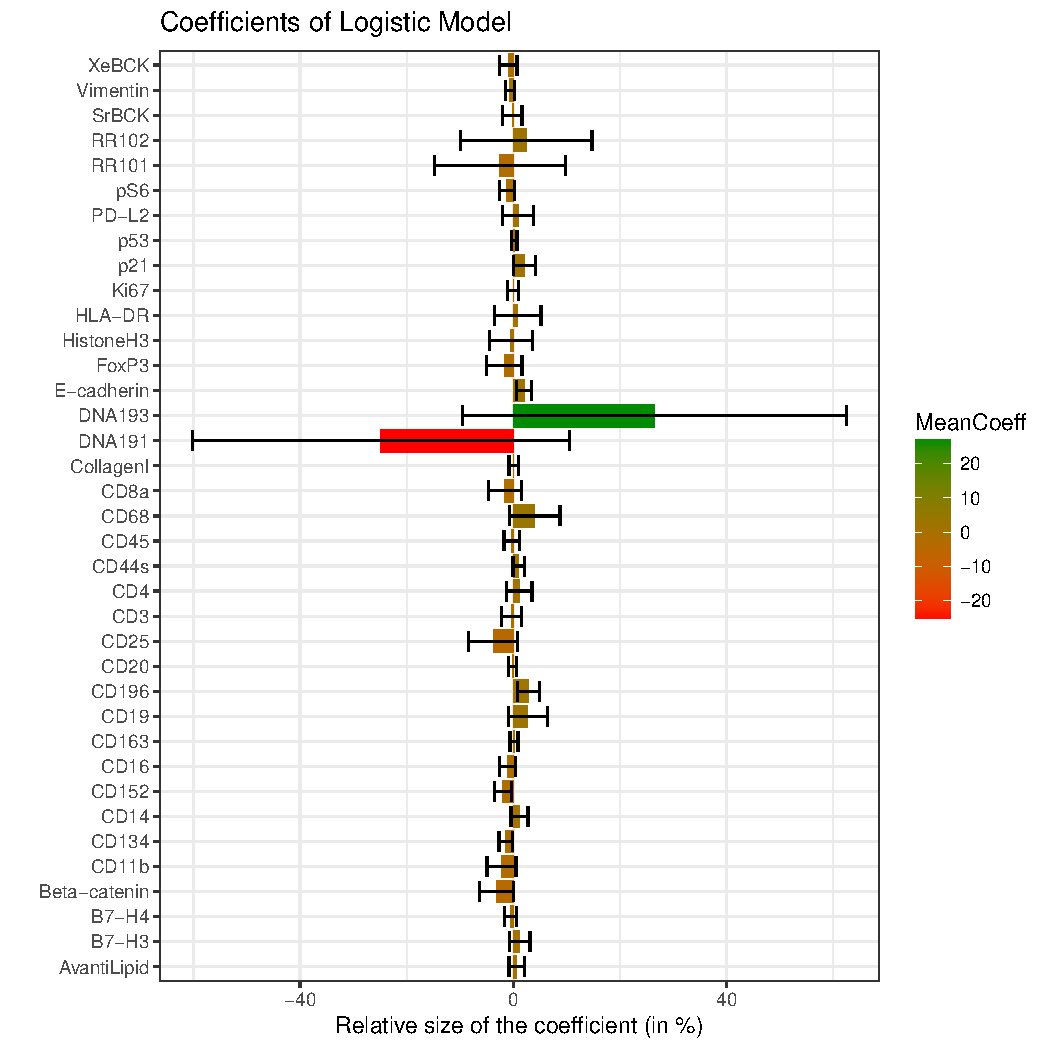
\includegraphics[width=\maxwidth]{figure/Fig_fullLogCoeff-1} \caption[Importance of the different stains according to the logistic model]{Importance of the different stains according to the logistic model.}\label{fig:Fig_fullLogCoeff}
\end{figure}


\end{knitrout}

This looks very similar to the LDA results (Figure \ref{fig:Fig_fullLogCoeff}). However, the error bars give a lot of additional insights. For LDA we had DNA191 and DNA193 also being very important, which was odd. Here we can see that while the coefficients of DNA191 and DNA193 are big, the uncertainty about them is also big. So, that it's not actually clear that they are important.

One result that was clear from the PCA was that there is a lot of correlation between the different stains. This is something that will influence a linear model. If there's strong correlation the model will struggle to distinguish between the influence of the different covariates (they all do the same thing) and so it becomes quite instable (See also: https://onlinecourses.science.psu.edu/stat501/node/346). To check for co-linearity, my MT5753 notes suggest to use ``variance inflation factors'' (VIF). These basically describe how well one covariate can be represented as a linear combination of the others. A VIF of greater than 5-10 is considered ``bad''.

VIFs can be calculated in R using the \texttt{car} library. Let's do it:
\begin{knitrout}
\definecolor{shadecolor}{rgb}{0.969, 0.969, 0.969}\color{fgcolor}\begin{kframe}
\begin{alltt}
\hlcom{# Co-linearity analysis}
\hlkwd{library}\hlstd{(car)}
\hlstd{vifVec} \hlkwb{=} \hlkwd{vif}\hlstd{(meanStain_LogitModel)}
\hlstd{vifVec[}\hlkwd{order}\hlstd{(vifVec,}\hlkwc{decreasing}\hlstd{=T)]}
\end{alltt}
\begin{verbatim}
##         DNA193         DNA191          RR102          RR101           CD68 
##    9974.633595    9643.717944    1294.106680    1293.076627     135.373597 
##       `HLA-DR`      HistoneH3          FoxP3 `Beta-catenin`           CD19 
##     134.685016      95.704941      82.279352      75.621073      74.025716 
##           CD25        `PD-L2`          CD11b           CD8a            CD4 
##      70.275328      64.014237      51.428826      50.404434      39.121114 
##        `B7-H3`            CD3            p21          CD196          XeBCK 
##      27.244525      26.236724      23.026496      22.649468      22.232085 
##          CD152          SrBCK    AvantiLipid           CD14           CD45 
##      21.834766      20.146580      17.454496      16.965421      15.643582 
##            pS6   `E-cadherin`           CD16        `B7-H4`           Ki67 
##      15.498719      14.284965      12.679932      10.612806       8.618162 
##          CD134          CD44s       Vimentin           CD20      CollagenI 
##       8.560725       5.902780       4.115182       3.910177       3.229387 
##          CD163            p53 
##       2.933174       1.743770
\end{verbatim}
\end{kframe}
\end{knitrout}

It seems like DNA193 and DNA191 seem to be strongly colinear and so do RR102 and RR101. This is nice given they're often just noise in the images and they also don't appear in the marker excel sheet. Let's remove them one at a time and see what it does.
\begin{knitrout}
\definecolor{shadecolor}{rgb}{0.969, 0.969, 0.969}\color{fgcolor}\begin{kframe}
\begin{alltt}
\hlcom{# Remove DNA193}
\hlstd{meanStainWide_Tranformed} \hlkwb{=} \hlstd{meanStainWide_Tranformed[,}\hlkwd{names}\hlstd{(meanStainWide_Tranformed)}\hlopt{!=}\hlstr{"DNA193"}\hlstd{]}
\hlcom{# Rerun the model}
\hlstd{meanStain_LogitModel} \hlkwb{=} \hlkwd{glm}\hlstd{(PtSnty} \hlopt{~}\hlstd{.,}\hlkwc{family}\hlstd{=}\hlkwd{binomial}\hlstd{(}\hlkwc{link}\hlstd{=}\hlstr{'logit'}\hlstd{),}
                           \hlkwc{data}\hlstd{=meanStainWide_Tranformed)}
\hlcom{# Check the VIFs}
\hlstd{vifVec} \hlkwb{=} \hlkwd{vif}\hlstd{(meanStain_LogitModel)}
\hlstd{vifVec[}\hlkwd{order}\hlstd{(vifVec,}\hlkwc{decreasing}\hlstd{=T)]}
\end{alltt}
\begin{verbatim}
##          RR102          RR101           CD68       `HLA-DR`          FoxP3 
##    1386.443436    1381.208303     131.122815     126.731151      84.410324 
##      HistoneH3           CD19           CD25 `Beta-catenin`        `PD-L2` 
##      78.778059      78.261591      76.789934      68.859995      53.075922 
##          CD11b           CD8a            CD4            CD3            p21 
##      48.620851      41.539153      33.102045      24.522113      24.082595 
##        `B7-H3`          XeBCK          CD152          CD196           CD14 
##      23.628003      18.312553      17.282496      16.306524      14.865896 
##    AvantiLipid            pS6           CD45          SrBCK   `E-cadherin` 
##      14.647060      14.201694      14.131115      13.175409      13.170279 
##         DNA191           CD16        `B7-H4`          CD134           Ki67 
##      11.554778      11.039728      10.537948       8.926170       8.105963 
##          CD44s       Vimentin           CD20      CollagenI          CD163 
##       5.671450       4.152301       3.746190       3.171522       2.706259 
##            p53 
##       1.817351
\end{verbatim}
\end{kframe}
\end{knitrout}

That brought DNA191 down, next let's take RR102.
\begin{knitrout}
\definecolor{shadecolor}{rgb}{0.969, 0.969, 0.969}\color{fgcolor}\begin{kframe}
\begin{alltt}
\hlcom{# Remove RR102}
\hlstd{meanStainWide_Tranformed} \hlkwb{=} \hlstd{meanStainWide_Tranformed[,}\hlkwd{names}\hlstd{(meanStainWide_Tranformed)}\hlopt{!=}\hlstr{"RR102"}\hlstd{]}
\hlcom{# Rerun the model}
\hlstd{meanStain_LogitModel} \hlkwb{=} \hlkwd{glm}\hlstd{(PtSnty} \hlopt{~}\hlstd{.,}\hlkwc{family}\hlstd{=}\hlkwd{binomial}\hlstd{(}\hlkwc{link}\hlstd{=}\hlstr{'logit'}\hlstd{),}
                           \hlkwc{data}\hlstd{=meanStainWide_Tranformed)}
\hlcom{# Check the VIFs}
\hlstd{vifVec} \hlkwb{=} \hlkwd{vif}\hlstd{(meanStain_LogitModel)}
\hlstd{vifVec[}\hlkwd{order}\hlstd{(vifVec,}\hlkwc{decreasing}\hlstd{=T)]}
\end{alltt}
\begin{verbatim}
##           CD68       `HLA-DR`          FoxP3           CD25           CD19 
##     131.124888     115.062156      81.406256      76.847966      76.775959 
##      HistoneH3 `Beta-catenin`        `PD-L2`          CD11b           CD8a 
##      71.431612      69.806026      48.977588      48.081861      37.743904 
##            CD4            CD3            p21        `B7-H3`          XeBCK 
##      31.145883      24.768951      24.629830      23.547026      17.425952 
##          CD152          CD196           CD14            pS6           CD45 
##      17.158307      15.325499      14.471240      14.191818      13.918672 
##    AvantiLipid   `E-cadherin`          SrBCK         DNA191           CD16 
##      13.528622      12.719828      12.333815      11.248299      10.740326 
##        `B7-H4`          RR101          CD134           Ki67          CD44s 
##      10.230362      10.151843       8.690677       7.949150       5.609450 
##       Vimentin           CD20      CollagenI          CD163            p53 
##       4.048068       3.615954       3.081919       2.681744       1.767517
\end{verbatim}
\end{kframe}
\end{knitrout}

Ok, now we're left with CD68. The linear discriminant analysis brought this up as an important contributer. However, it seems to be quite strongly co-linear with other markers. Perhaps this is because CD68 is a generic Monocyte/Macrophage marker which is also captured by other markers. Mhm, let's actually check this and see what correlates most strongly with CD68.

\begin{knitrout}
\definecolor{shadecolor}{rgb}{0.969, 0.969, 0.969}\color{fgcolor}\begin{kframe}
\begin{alltt}
\hlstd{cd68CoLinModel} \hlkwb{=} \hlkwd{lm}\hlstd{(CD68}\hlopt{~}\hlstd{.,}
                    \hlkwc{data}\hlstd{=meanStainWide_Tranformed[,}\hlkwd{names}\hlstd{(meanStainWide_Tranformed)}\hlopt{!=}\hlstr{"PtSnty"}\hlstd{])}
\hlkwd{summary}\hlstd{(cd68CoLinModel)}
\end{alltt}
\begin{verbatim}
## 
## Call:
## lm(formula = CD68 ~ ., data = meanStainWide_Tranformed[, names(meanStainWide_Tranformed) != 
##     "PtSnty"])
## 
## Residuals:
##      Min       1Q   Median       3Q      Max 
## -0.28093 -0.07238 -0.02345  0.06982  0.41295 
## 
## Coefficients:
##                  Estimate Std. Error t value Pr(>|t|)    
## (Intercept)    -2.535e-17  1.383e-02   0.000   1.0000    
## SrBCK          -8.359e-04  4.012e-02  -0.021   0.9834    
## RR101           2.316e-02  3.068e-02   0.755   0.4524    
## AvantiLipid     4.071e-04  3.734e-02   0.011   0.9913    
## XeBCK           1.629e-02  4.159e-02   0.392   0.6962    
## CD196          -2.097e-04  3.768e-02  -0.006   0.9956    
## CD19           -1.371e-02  3.572e-02  -0.384   0.7019    
## Vimentin        1.990e-02  2.513e-02   0.792   0.4306    
## CD163          -1.697e-02  2.322e-02  -0.731   0.4667    
## CD20            6.658e-03  2.326e-02   0.286   0.7754    
## CD16           -3.035e-02  3.513e-02  -0.864   0.3900    
## CD25           -1.162e-03  4.464e-02  -0.026   0.9793    
## p53            -1.547e-02  1.663e-02  -0.930   0.3549    
## CD134           1.480e-02  2.577e-02   0.574   0.5672    
## CD45           -4.463e-02  3.253e-02  -1.372   0.1736    
## CD44s          -1.255e-02  2.251e-02  -0.557   0.5787    
## CD14           -2.894e-02  3.703e-02  -0.781   0.4367    
## FoxP3           1.017e-01  9.420e-02   1.080   0.2832    
## CD4            -5.397e-02  5.316e-02  -1.015   0.3128    
## `E-cadherin`    1.531e-02  3.053e-02   0.502   0.6172    
## p21             4.827e-02  4.028e-02   1.198   0.2341    
## CD152          -1.202e-01  3.617e-02  -3.324   0.0013 ** 
## CD8a            3.378e-01  4.867e-02   6.940 6.97e-10 ***
## CD11b           2.801e-01  6.254e-02   4.478 2.30e-05 ***
## `Beta-catenin`  3.427e-02  6.445e-02   0.532   0.5963    
## `B7-H4`         2.850e-03  3.163e-02   0.090   0.9284    
## Ki67           -2.432e-02  2.951e-02  -0.824   0.4121    
## CollagenI      -5.288e-03  2.579e-02  -0.205   0.8380    
## CD3             1.609e-01  5.439e-02   2.958   0.0040 ** 
## `PD-L2`        -9.746e-03  6.929e-02  -0.141   0.8885    
## `B7-H3`        -2.678e-02  5.107e-02  -0.524   0.6013    
## `HLA-DR`        2.126e-01  1.265e-01   1.680   0.0965 .  
## pS6            -2.772e-02  3.547e-02  -0.781   0.4368    
## HistoneH3       2.280e-01  9.785e-02   2.330   0.0221 *  
## DNA191         -2.881e-02  3.213e-02  -0.897   0.3724    
## ---
## Signif. codes:  0 '***' 0.001 '**' 0.01 '*' 0.05 '.' 0.1 ' ' 1
## 
## Residual standard error: 0.1521 on 86 degrees of freedom
## Multiple R-squared:  0.9834,	Adjusted R-squared:  0.9769 
## F-statistic: 149.9 on 34 and 86 DF,  p-value: < 2.2e-16
\end{verbatim}
\end{kframe}
\end{knitrout}

So, the following correlate with CD68 (descriptions taken from the excel sheet):
\begin{itemize}
  \item CD8a (p$<$1e-10): Marker of cytotoxic T cells
  \item CD11b (p$<$1e-5): Integrin alpha M(ITGAM). $\alpha$M$\beta$2 is expressed on the surface of many leukocytes involved in the innate immune system, including monocytes, granulocytes, macrophages, and natural killer cells.
  \item CD152 (p$<$1e-2): Check point inhibitor protein.
  \item CD3 (p$<$1e-2): General T Cell Marker
  \item HistoneH3 (p$<$5e-2): Generic Cell Marker
\end{itemize}

The correlation with t-cell markers is interesting. Perhaps this reflects a general immune response? If there are a lot of macrophages there are also a lot of t-cells? The check point inhibitor is kind of weird. Is this checkpoint inhibitor maybe only expressed on macrohpages?

No, according to Wikipedia it's expressed on t-cells. So, I guess that goes with the t-cell theme.

At this point it's a bit difficult to tell which marker to drop. I'm hesitant to drop cd68 all together, since I like it as a macrophage marker. I also don't want to drop the t-cell markers, if I don't have to. The one that seems to contain the least extra information is CD11b, as it's simply a generic immune marker. Let's drop this for now and revise later if this seems not appropriate.
\begin{knitrout}
\definecolor{shadecolor}{rgb}{0.969, 0.969, 0.969}\color{fgcolor}\begin{kframe}
\begin{alltt}
\hlcom{# Remove CD11b}
\hlstd{meanStainWide_Tranformed} \hlkwb{=} \hlstd{meanStainWide_Tranformed[,}\hlkwd{names}\hlstd{(meanStainWide_Tranformed)}\hlopt{!=}\hlstr{"CD11b"}\hlstd{]}
\hlcom{# Rerun the model}
\hlstd{meanStain_LogitModel} \hlkwb{=} \hlkwd{glm}\hlstd{(PtSnty} \hlopt{~}\hlstd{.,}\hlkwc{family}\hlstd{=}\hlkwd{binomial}\hlstd{(}\hlkwc{link}\hlstd{=}\hlstr{'logit'}\hlstd{),}
                           \hlkwc{data}\hlstd{=meanStainWide_Tranformed)}
\hlcom{# Check the VIFs}
\hlstd{vifVec} \hlkwb{=} \hlkwd{vif}\hlstd{(meanStain_LogitModel)}
\hlstd{vifVec[}\hlkwd{order}\hlstd{(vifVec,}\hlkwc{decreasing}\hlstd{=T)]}
\end{alltt}
\begin{verbatim}
##       `HLA-DR`          FoxP3           CD68      HistoneH3           CD25 
##     127.878532      79.976460      79.099776      72.121253      66.447028 
##           CD19 `Beta-catenin`        `PD-L2`           CD8a            CD3 
##      66.340546      56.781593      44.204763      30.834055      25.196556 
##            CD4        `B7-H3`            p21          CD152          XeBCK 
##      24.227790      21.764014      20.585890      17.219077      16.892651 
##          CD196    AvantiLipid   `E-cadherin`           CD14           CD45 
##      13.976792      12.885859      12.833327      12.540062      11.777482 
##          SrBCK            pS6           CD16         DNA191          RR101 
##      11.538345      10.881197      10.521985       9.588140       8.411429 
##        `B7-H4`          CD134           Ki67          CD44s       Vimentin 
##       7.924068       7.233788       7.133291       5.420239       3.552679 
##           CD20      CollagenI          CD163            p53 
##       3.336951       3.085309       2.912598       1.732963
\end{verbatim}
\end{kframe}
\end{knitrout}

Mhm, at this point there's still a fair bit of co-linearity. I could continue removing stains using biological reasoning, but it seems more thorough to do a sweep through all possible combinations of these variables and use that to decide which are the ones that contain the most information.

% =======================================================
% ---- Naive Logistic Model -----
\section{Sweep through Models with No Interactions}
The \texttt{sweep()} function allows to do ``model optimisation''. By default it takes the input model, tries to add or remove one covariates at a time and chooses the one option that gives the best improvement in AIC (it does not consider interaction terms). Let's try that here:
\begin{knitrout}
\definecolor{shadecolor}{rgb}{0.969, 0.969, 0.969}\color{fgcolor}\begin{kframe}
\begin{alltt}
\hlcom{# Start with the raw data again}
\hlstd{meanStainWide_Tranformed} \hlkwb{=} \hlstd{meanStain_Wide}
\hlstd{preprocessParams} \hlkwb{=} \hlkwd{preProcess}\hlstd{(meanStain_Wide[,}\hlnum{3}\hlopt{:}\hlkwd{dim}\hlstd{(meanStain_Wide)[}\hlnum{2}\hlstd{]],}
                              \hlkwc{method}\hlstd{=}\hlkwd{c}\hlstd{(}\hlstr{"center"}\hlstd{,} \hlstr{"scale"}\hlstd{),}\hlkwc{verbose}\hlstd{=T)}
\end{alltt}
\begin{verbatim}
## Calculating 37 means for centering
## Calculating 37 standard deviations for scaling
\end{verbatim}
\begin{alltt}
\hlstd{meanStainWide_Tranformed[,}\hlnum{3}\hlopt{:}\hlkwd{dim}\hlstd{(meanStain_Wide)[}\hlnum{2}\hlstd{]]} \hlkwb{=}
  \hlkwd{predict}\hlstd{(preprocessParams, meanStain_Wide[,}\hlnum{3}\hlopt{:}\hlkwd{dim}\hlstd{(meanStain_Wide)[}\hlnum{2}\hlstd{]])}

\hlcom{# Remove the coreId column so that it doesn't influence the analysis}
\hlstd{meanStainWide_Tranformed} \hlkwb{=} \hlkwd{cbind}\hlstd{(meanStainWide_Tranformed}\hlopt{$}\hlstd{PtSnty,}
                                 \hlstd{meanStainWide_Tranformed[,}\hlnum{3}\hlopt{:}\hlkwd{ncol}\hlstd{(meanStainWide_Tranformed)])}
\hlkwd{names}\hlstd{(meanStainWide_Tranformed)} \hlkwb{=} \hlkwd{c}\hlstd{(}\hlstr{"PtSnty"}\hlstd{,markerLabelsVec)}

\hlcom{# Remove RR102, DNA193 and CD11b because of their high correlation}
\hlstd{meanStainWide_LessCorr} \hlkwb{=} \hlstd{meanStainWide_Tranformed[,}
                      \hlopt{!}\hlstd{(}\hlkwd{names}\hlstd{(meanStainWide_Tranformed)} \hlopt \hlkwd{c}\hlstd{(}\hlstr{"DNA193"}\hlstd{,}\hlstr{"RR102"}\hlstd{,}\hlstr{"CD11b"}\hlstd{))]}

\hlcom{# Do step-wise model optimisation}
\hlstd{initModel} \hlkwb{=} \hlkwd{glm}\hlstd{(PtSnty} \hlopt{~}\hlstd{.,}\hlkwc{family}\hlstd{=}\hlkwd{binomial}\hlstd{(}\hlkwc{link}\hlstd{=}\hlstr{'logit'}\hlstd{),}
                           \hlkwc{data}\hlstd{=meanStainWide_LessCorr)}
\hlstd{naiveStepSearch} \hlkwb{=} \hlkwd{step}\hlstd{(initModel,}\hlkwc{trace}\hlstd{=}\hlnum{0}\hlstd{)}
\hlstd{naiveStepSearch}\hlopt{$}\hlstd{anova}
\end{alltt}
\begin{verbatim}
##             Step Df    Deviance Resid. Df Resid. Dev      AIC
## 1                NA          NA        86   86.91700 156.9170
## 2        - RR101  1 0.001332371        87   86.91833 154.9183
## 3  - AvantiLipid  1 0.004097164        88   86.92243 152.9224
## 4          - CD4  1 0.005426860        89   86.92785 150.9279
## 5         - Ki67  1 0.021675203        90   86.94953 148.9495
## 6         - CD20  1 0.032426262        91   86.98195 146.9820
## 7    - CollagenI  1 0.043633873        92   87.02559 145.0256
## 8      - `B7-H4`  1 0.250802923        93   87.27639 143.2764
## 9          - CD3  1 0.432061307        94   87.70845 141.7085
## 10   - HistoneH3  1 0.403668240        95   88.11212 140.1121
## 11    - `HLA-DR`  1 0.422713382        96   88.53483 138.5348
## 12       - XeBCK  1 0.295849902        97   88.83068 136.8307
## 13       - SrBCK  1 0.972272480        98   89.80296 135.8030
## 14         - p53  1 0.645405234        99   90.44836 134.4484
## 15        - CD45  1 1.582480439       100   92.03084 134.0308
## 16     - `B7-H3`  1 1.183532376       101   93.21437 133.2144
\end{verbatim}
\end{kframe}
\end{knitrout}

The results are interesting. It removes almost all the ``non-indicative stains'' (It removes RR101, AvantiLipid, XeBCK, SrBCK). The other stains it removes seem kind of generic:
\begin{itemize}
  \item CD4: found on the surface of immune cells such as T helper cells, monocytes, macrophages, and dendritic cells.
  \item Ki67: marker of cell proliferation
  \item CD20: B Cell Marker
  \item CollagenI: part of the extracellular matrix.
  \item B7-H4: immune checkpoint protein expressed on the surface of antigen presenting cells
  \item CD3 (p$<$1e-2): General T Cell Marker
  \item HistoneH3 (p$<$5e-2): Generic Cell Marker
  \item HLA-DR: HLA-DR is an MHC class II cell surface receptor on antigen presenting cells. Upregulation can indicate immune stimulation (wikipedia)
  \item p53: involved in DNA repair. 70-90\% of ovarian tumors have mutated p53
  \item CD45: Protein tyrosine phosphatase, receptor type, C. Common antigen on leukocytes
  \item B7-H3: immune checkpoint protein
\end{itemize}

But it does leave DNA191 in! Also, these results have to be taken with a bit of a grain of salt: Which stains I remove is to some extend arbitrary, when looking at the detailed output of the stepping search often many stains would give the same final output. It would be good to do this stepping with a biologist who knows which stains would be interesting/useful to keep! Similarly, the results of what's in the final model depends on what I start with. If I don't remove DNA191 the results are different:
\begin{knitrout}
\definecolor{shadecolor}{rgb}{0.969, 0.969, 0.969}\color{fgcolor}\begin{kframe}
\begin{alltt}
\hlstd{initModel} \hlkwb{=} \hlkwd{glm}\hlstd{(PtSnty} \hlopt{~}\hlstd{.,}\hlkwc{family}\hlstd{=}\hlkwd{binomial}\hlstd{(}\hlkwc{link}\hlstd{=}\hlstr{'logit'}\hlstd{),}
                           \hlkwc{data}\hlstd{=meanStainWide_Tranformed)}
\hlstd{naiveStepSearch_Full} \hlkwb{=} \hlkwd{step}\hlstd{(initModel,}\hlkwc{trace}\hlstd{=}\hlnum{0}\hlstd{)}
\hlstd{naiveStepSearch_Full}\hlopt{$}\hlstd{anova}
\end{alltt}
\begin{verbatim}
##             Step Df    Deviance Resid. Df Resid. Dev      AIC
## 1                NA          NA        83   80.93421 156.9342
## 2         - Ki67  1 0.007225489        84   80.94143 154.9414
## 3    - CollagenI  1 0.031036492        85   80.97247 152.9725
## 4        - SrBCK  1 0.053739333        86   81.02621 151.0262
## 5    - HistoneH3  1 0.095541764        87   81.12175 149.1218
## 6          - CD3  1 0.084265636        88   81.20602 147.2060
## 7     - `HLA-DR`  1 0.114334599        89   81.32035 145.3204
## 8        - CD163  1 0.232541900        90   81.55289 143.5529
## 9        - RR101  1 0.252665414        91   81.80556 141.8056
## 10       - RR102  1 0.004343968        92   81.80990 139.8099
## 11        - CD45  1 0.274712590        93   82.08462 138.0846
## 12         - p53  1 0.695679860        94   82.78029 136.7803
## 13     - `PD-L2`  1 0.870849737        95   83.65114 135.6511
## 14 - AvantiLipid  1 1.271694659        96   84.92284 134.9228
## 15       - FoxP3  1 0.937781343        97   85.86062 133.8606
## 16         - CD4  1 0.484753536        98   86.34537 132.3454
## 17        - CD8a  1 0.895501618        99   87.24088 131.2409
## 18       - XeBCK  1 1.656620892       100   88.89750 130.8975
## 19        - CD14  1 1.821697731       101   90.71919 130.7192
## 20        - CD20  1 1.434197238       102   92.15339 130.1534
\end{verbatim}
\end{kframe}
\end{knitrout}

Weirdly this keeps both DNA stains and has a lower AIC. But it throws out more of the normal stains, and still has the VIF problem:
\begin{knitrout}
\definecolor{shadecolor}{rgb}{0.969, 0.969, 0.969}\color{fgcolor}\begin{kframe}
\begin{alltt}
\hlstd{vifVec} \hlkwb{=} \hlkwd{vif}\hlstd{(naiveStepSearch_Full)}
\hlstd{vifVec[}\hlkwd{order}\hlstd{(vifVec,}\hlkwc{decreasing}\hlstd{=T)]}
\end{alltt}
\begin{verbatim}
##         DNA193         DNA191           CD68           CD19           CD25 
##    2473.765129    2408.801747      27.507171      24.599355      23.023923 
## `Beta-catenin`          CD11b        `B7-H3`            p21   `E-cadherin` 
##      21.793794      14.012134      11.758702       8.813599       7.911414 
##          CD196          CD152        `B7-H4`            pS6           CD16 
##       6.953314       6.921268       5.854936       5.332492       5.175765 
##          CD134          CD44s       Vimentin 
##       4.525887       2.406563       2.149317
\end{verbatim}
\end{kframe}
\end{knitrout}

In contrast, the reduced model with DNA193 removed looks better:
\begin{knitrout}
\definecolor{shadecolor}{rgb}{0.969, 0.969, 0.969}\color{fgcolor}\begin{kframe}
\begin{alltt}
\hlstd{vifVec} \hlkwb{=} \hlkwd{vif}\hlstd{(naiveStepSearch)}
\hlstd{vifVec[}\hlkwd{order}\hlstd{(vifVec,}\hlkwc{decreasing}\hlstd{=T)]}
\end{alltt}
\begin{verbatim}
##           CD25           CD19 `Beta-catenin`        `PD-L2`           CD68 
##      53.897381      49.921858      31.307486      24.661024      24.516927 
##          FoxP3           CD8a            p21          CD152           CD16 
##      15.895193      13.364489      11.621150       8.730938       8.649581 
##   `E-cadherin`           CD14          CD196            pS6          CD134 
##       7.329475       6.376292       6.343065       5.307749       4.443304 
##          CD163         DNA191          CD44s       Vimentin 
##       3.676132       3.522567       2.488889       2.195531
\end{verbatim}
\end{kframe}
\end{knitrout}

Though still not great... Nevertheless I will focus on this model (the one with only DNA191) for now. Let's plot the coefficients again.
\begin{knitrout}
\definecolor{shadecolor}{rgb}{0.969, 0.969, 0.969}\color{fgcolor}\begin{kframe}
\begin{alltt}
\hlstd{confLevel} \hlkwb{=} \hlnum{0.95} \hlcom{# Statistical confidence indicated by error bars}

\hlstd{PlotCoefficients} \hlkwb{=} \hlkwa{function}\hlstd{(}\hlkwc{model}\hlstd{,}\hlkwc{confLevel}\hlstd{=}\hlnum{0.95}\hlstd{,}\hlkwc{yLim}\hlstd{=}\hlkwd{c}\hlstd{(}\hlopt{-}\hlnum{25}\hlstd{,}\hlnum{25}\hlstd{),}\hlkwc{yPos}\hlstd{=}\hlnum{20}\hlstd{,}\hlkwc{starSize}\hlstd{=}\hlnum{7}\hlstd{,}\hlkwc{errBarWidth}\hlstd{=}\hlnum{.8}\hlstd{) \{}
  \hlstd{logitMCoeffs} \hlkwb{=} \hlstd{model}\hlopt{$}\hlstd{coefficients}
  \hlstd{logitMStdErrs} \hlkwb{=} \hlkwd{summary}\hlstd{(model)}\hlopt{$}\hlstd{coefficients[,}\hlnum{2}\hlstd{]}

  \hlcom{# Normalise}
  \hlstd{normFact} \hlkwb{=} \hlkwd{sum}\hlstd{(}\hlkwd{abs}\hlstd{(logitMCoeffs))}
  \hlstd{logitMCoeffs} \hlkwb{=} \hlstd{logitMCoeffs}\hlopt{*}\hlnum{100}\hlopt{/}\hlstd{normFact}
  \hlstd{logitMStdErrs} \hlkwb{=} \hlstd{logitMStdErrs}\hlopt{*}\hlnum{100}\hlopt{/}\hlstd{normFact}
  \hlstd{confIntLogitCoeffs} \hlkwb{=} \hlkwd{data.frame}\hlstd{(}\hlkwc{MarkerLabels}\hlstd{=}\hlkwd{names}\hlstd{(logitMCoeffs)[}\hlnum{2}\hlopt{:}\hlkwd{length}\hlstd{(logitMCoeffs)],}
                                  \hlkwc{MeanCoeff}\hlstd{=}\hlkwd{as.numeric}\hlstd{(logitMCoeffs[}\hlnum{2}\hlopt{:}\hlkwd{length}\hlstd{(logitMCoeffs)]),}
                                  \hlkwc{SE}\hlstd{=logitMStdErrs[}\hlnum{2}\hlopt{:}\hlkwd{length}\hlstd{(logitMStdErrs)],}
                                  \hlkwc{CI}\hlstd{=}\hlkwd{rep}\hlstd{(}\hlnum{0}\hlstd{,}\hlkwd{length}\hlstd{(logitMStdErrs[}\hlnum{2}\hlopt{:}\hlkwd{length}\hlstd{(logitMStdErrs)])))}

  \hlcom{# Compute the confidence interval}
  \hlstd{nSamples} \hlkwb{=} \hlkwd{nrow}\hlstd{(meanStainWide_Tranformed)}
  \hlstd{confIntLogitCoeffs}\hlopt{$}\hlstd{CI} \hlkwb{=} \hlkwd{qt}\hlstd{(confLevel}\hlopt{/}\hlnum{2}\hlopt{+}\hlnum{.5}\hlstd{,nSamples)}\hlopt{*}\hlstd{confIntLogitCoeffs}\hlopt{$}\hlstd{SE}

  \hlcom{# Order by size of contribution}
  \hlstd{confIntLogitCoeffs}\hlopt{$}\hlstd{MarkerLabels} \hlkwb{=} \hlkwd{factor}\hlstd{(confIntLogitCoeffs}\hlopt{$}\hlstd{MarkerLabels,}
                                           \hlkwc{levels} \hlstd{= confIntLogitCoeffs}\hlopt{$}\hlstd{MarkerLabels[}
                                             \hlkwd{order}\hlstd{(confIntLogitCoeffs}\hlopt{$}\hlstd{MeanCoeff,}\hlkwc{decreasing}\hlstd{=F)}
                                           \hlstd{])}

  \hlcom{# Plot}
  \hlstd{p}\hlkwb{=}\hlkwd{ggplot}\hlstd{(confIntLogitCoeffs,}\hlkwd{aes}\hlstd{(}\hlkwc{x}\hlstd{=MarkerLabels,}\hlkwc{y}\hlstd{=MeanCoeff,}\hlkwc{fill}\hlstd{=MeanCoeff))} \hlopt{+}
    \hlkwd{geom_bar}\hlstd{(}\hlkwc{position}\hlstd{=}\hlkwd{position_dodge}\hlstd{(}\hlnum{0.9}\hlstd{),} \hlkwc{stat}\hlstd{=}\hlstr{"identity"}\hlstd{)} \hlopt{+}
    \hlkwd{geom_errorbar}\hlstd{(}\hlkwd{aes}\hlstd{(}\hlkwc{ymin}\hlstd{=MeanCoeff}\hlopt{-}\hlstd{CI,} \hlkwc{ymax}\hlstd{=MeanCoeff}\hlopt{+}\hlstd{CI),}
                  \hlkwc{width}\hlstd{=errBarWidth,}                    \hlcom{# Width of the error bars}
                  \hlkwc{position}\hlstd{=}\hlkwd{position_dodge}\hlstd{(}\hlnum{0.9}\hlstd{))} \hlopt{+}
    \hlkwd{theme_bw}\hlstd{()} \hlopt{+}
    \hlkwd{ylim}\hlstd{(yLim)} \hlopt{+}
    \hlkwd{ylab}\hlstd{(}\hlstr{"Relative size of the coefficient (in %)"}\hlstd{)} \hlopt{+}
    \hlkwd{xlab}\hlstd{(}\hlstr{""}\hlstd{)} \hlopt{+}
    \hlkwd{scale_fill_gradient}\hlstd{(}\hlkwc{low}\hlstd{=}\hlstr{"red"}\hlstd{,}\hlkwc{high}\hlstd{=}\hlstr{"green4"}\hlstd{)} \hlopt{+}
    \hlkwd{ggtitle}\hlstd{(}\hlkwd{paste}\hlstd{(}\hlstr{"Coefficients of Reduced Logistic Model"}\hlstd{,}\hlkwc{sep}\hlstd{=}\hlstr{""}\hlstd{))}

  \hlcom{# Add stars to indicate significance}
  \hlstd{pValVec} \hlkwb{=} \hlkwd{summary}\hlstd{(model)}\hlopt{$}\hlstd{coefficients[,}\hlnum{4}\hlstd{]}
  \hlkwa{for}\hlstd{(marker} \hlkwa{in} \hlstd{confIntLogitCoeffs}\hlopt{$}\hlstd{MarkerLabels) \{}
    \hlkwa{if} \hlstd{(pValVec[marker]} \hlopt{<} \hlnum{0.01}\hlstd{) \{}
      \hlstd{p} \hlkwb{=} \hlstd{p} \hlopt{+} \hlkwd{annotate}\hlstd{(}\hlstr{"text"}\hlstd{,} \hlkwc{x} \hlstd{= marker,} \hlkwc{y} \hlstd{= yPos,}
                       \hlkwc{label} \hlstd{=} \hlstr{"**"}\hlstd{,} \hlkwc{size} \hlstd{= starSize)}
    \hlstd{\}} \hlkwa{else if} \hlstd{(pValVec[marker]} \hlopt{<} \hlnum{0.05}\hlstd{) \{}
      \hlstd{p} \hlkwb{=} \hlstd{p} \hlopt{+} \hlkwd{annotate}\hlstd{(}\hlstr{"text"}\hlstd{,} \hlkwc{x} \hlstd{= marker,} \hlkwc{y} \hlstd{= yPos,}
                       \hlkwc{label} \hlstd{=} \hlstr{"*"}\hlstd{,} \hlkwc{size} \hlstd{= starSize)}
    \hlstd{\}}
  \hlstd{\}}

  \hlcom{# Flip the axes}
  \hlstd{p} \hlkwb{=} \hlstd{p} \hlopt{+} \hlkwd{coord_flip}\hlstd{()}
  \hlkwd{return}\hlstd{(p)}
\hlstd{\}}
\hlkwd{PlotCoefficients}\hlstd{(naiveStepSearch)}
\end{alltt}
\end{kframe}\begin{figure}[t]
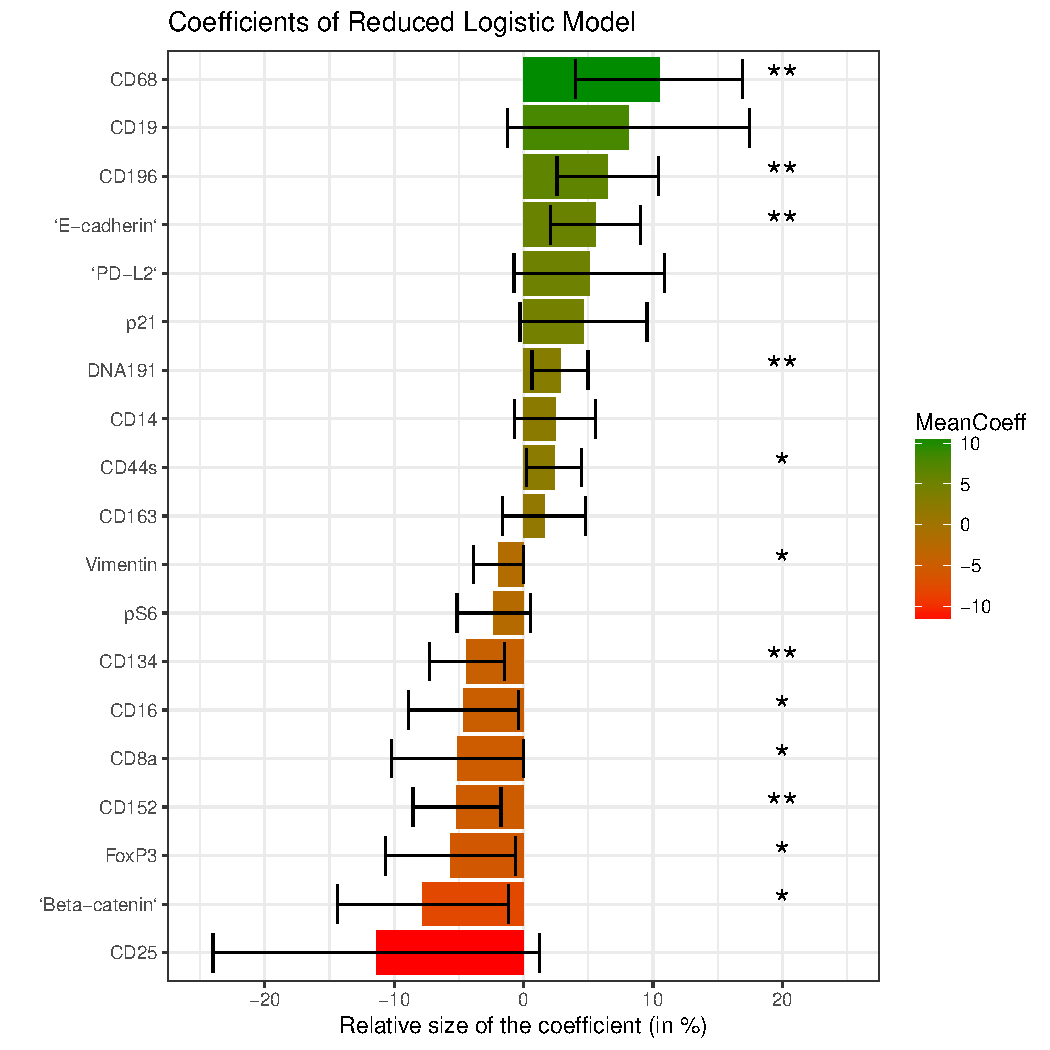
\includegraphics[width=\maxwidth]{figure/Fig_redModCoeff-1} \caption[Importance of the different stains according to the reduced logistic model]{Importance of the different stains according to the reduced logistic model. Asterisk indicates level of statistical support for non-zero contribution from this stain (T-test: *p$<$0.05,**p$<$0.01).}\label{fig:Fig_redModCoeff}
\end{figure}


\end{knitrout}

\section{Cross Validation}
Deviance is one way of evaluating our models, however, it's  somewhat difficult to interpret. Since we are trying to build a classifier, an idea of the models accuracy in predicting unseen patients would be a more intuitive and useful number. Thus, let's do a cross-validation test, to see how well our models classify. First make a function to do v-fold cross classification on the data:
\begin{knitrout}
\definecolor{shadecolor}{rgb}{0.969, 0.969, 0.969}\color{fgcolor}\begin{kframe}
\begin{alltt}
\hlcom{# Function to do a v-fold cross validations (v different ways of splitting}
\hlcom{# the data into training and testing). This code is adopted from:}
\hlcom{# https://www.stat.berkeley.edu/~s133/Class2a.html}

\hlstd{LogisticCrossVal} \hlkwb{=} \hlkwa{function}\hlstd{(}\hlkwc{nIter}\hlstd{,}\hlkwc{v}\hlstd{,}\hlkwc{formula}\hlstd{,}\hlkwc{data}\hlstd{)\{}
  \hlstd{accuracyVec} \hlkwb{=} \hlkwd{rep}\hlstd{(}\hlnum{0}\hlstd{,nIter)}
  \hlkwa{for} \hlstd{(i} \hlkwa{in} \hlkwd{seq}\hlstd{(nIter)) \{}
    \hlcom{# Split the data into training and testing.}
    \hlcom{# It will assign each core into one of nFold groups. When it's this folds turn}
    \hlcom{# the cores in this fold will be the testing set.}
    \hlstd{nSamples} \hlkwb{=} \hlkwd{nrow}\hlstd{(meanStainWide_Tranformed)}
    \hlstd{grps} \hlkwb{=} \hlkwd{cut}\hlstd{(}\hlnum{1}\hlopt{:}\hlstd{nSamples,nFolds,}\hlkwc{labels}\hlstd{=}\hlnum{FALSE}\hlstd{)[}\hlkwd{sample}\hlstd{(}\hlnum{1}\hlopt{:}\hlstd{nSamples)]}

    \hlcom{# Do the validation}
    \hlstd{pred} \hlkwb{=} \hlkwd{lapply}\hlstd{(}\hlnum{1}\hlopt{:}\hlstd{nFolds,}\hlkwa{function}\hlstd{(}\hlkwc{i}\hlstd{,}\hlkwc{formula}\hlstd{,}\hlkwc{data}\hlstd{)\{}
            \hlstd{omit} \hlkwb{=} \hlkwd{which}\hlstd{(grps} \hlopt{==} \hlstd{i)}
          \hlstd{z} \hlkwb{=} \hlkwd{glm}\hlstd{(formula,}\hlkwc{family}\hlstd{=}\hlkwd{binomial}\hlstd{(}\hlkwc{link}\hlstd{=}\hlstr{'logit'}\hlstd{),}\hlkwc{data}\hlstd{=data[}\hlopt{-}\hlstd{omit,])}
          \hlstd{predictions} \hlkwb{=} \hlkwd{predict}\hlstd{(z,data[omit,],}\hlkwc{type}\hlstd{=}\hlstr{'response'}\hlstd{)}
          \hlstd{predictions} \hlkwb{=} \hlkwd{ifelse}\hlstd{(predictions} \hlopt{>} \hlnum{0.5}\hlstd{,}\hlnum{1}\hlstd{,}\hlnum{0}\hlstd{)}
          \hlstd{ClasificError} \hlkwb{=} \hlnum{1}\hlopt{-}\hlkwd{mean}\hlstd{(predictions} \hlopt{!=} \hlstd{data[omit,]}\hlopt{$}\hlstd{PtSnty)}
            \hlstd{\},formula,data)}

    \hlstd{accuracyVec[i]} \hlkwb{=} \hlkwd{mean}\hlstd{(}\hlkwd{unlist}\hlstd{(pred))}
  \hlstd{\}}

  \hlkwd{return}\hlstd{(accuracyVec)}
\hlstd{\}}
\end{alltt}
\end{kframe}
\end{knitrout}
And now apply it:
\begin{knitrout}
\definecolor{shadecolor}{rgb}{0.969, 0.969, 0.969}\color{fgcolor}\begin{kframe}
\begin{alltt}
\hlstd{nIter} \hlkwb{=} \hlnum{100}
\hlstd{nFolds} \hlkwb{=} \hlnum{5}

\hlcom{# Do the cross validation}
\hlstd{fullModAccVec} \hlkwb{=} \hlkwd{LogisticCrossVal}\hlstd{(nIter,nFolds,meanStain_LogitModel}\hlopt{$}\hlstd{formula,}
                                 \hlstd{meanStainWide_Tranformed)}
\hlstd{redModAccVec} \hlkwb{=} \hlkwd{LogisticCrossVal}\hlstd{(nIter,nFolds,naiveStepSearch}\hlopt{$}\hlstd{formula,}
                                \hlstd{meanStainWide_Tranformed)}
\hlstd{redModAccVec_BothDNAs} \hlkwb{=} \hlkwd{LogisticCrossVal}\hlstd{(nIter,nFolds,naiveStepSearch_Full}\hlopt{$}\hlstd{formula,}
                                         \hlstd{meanStainWide_Tranformed)}

\hlcom{# Plot the results}
\hlstd{xValidResult} \hlkwb{=} \hlkwd{data.frame}\hlstd{(}\hlkwc{Accuracy}\hlstd{=}\hlkwd{c}\hlstd{(fullModAccVec,redModAccVec,redModAccVec_BothDNAs),}
                          \hlkwc{Model}\hlstd{=}\hlkwd{as.factor}\hlstd{(}\hlkwd{c}\hlstd{(}\hlkwd{rep}\hlstd{(}\hlnum{0}\hlstd{,nIter),}\hlkwd{rep}\hlstd{(}\hlnum{1}\hlstd{,nIter),}\hlkwd{rep}\hlstd{(}\hlnum{2}\hlstd{,nIter))))}
\hlkwd{ggplot}\hlstd{(xValidResult,}\hlkwd{aes}\hlstd{(}\hlkwc{x}\hlstd{=Model,}\hlkwc{y}\hlstd{=Accuracy,}\hlkwc{fill}\hlstd{=Model))} \hlopt{+}
  \hlkwd{geom_boxplot}\hlstd{()} \hlopt{+}
  \hlkwd{xlab}\hlstd{(}\hlstr{""}\hlstd{)} \hlopt{+}
  \hlkwd{scale_fill_discrete}\hlstd{(}\hlkwc{breaks}\hlstd{=}\hlkwd{seq}\hlstd{(}\hlnum{0}\hlstd{,}\hlnum{2}\hlstd{),}\hlkwc{labels}\hlstd{=}\hlkwd{c}\hlstd{(}\hlstr{"Model based\textbackslash{}n on all stains"}\hlstd{,}
                                               \hlstr{"Reduced Model"}\hlstd{,}
                                               \hlstr{"Reduced Model\textbackslash{}n with DNA191\textbackslash{}n and DNA193"}\hlstd{))}
\end{alltt}
\end{kframe}\begin{figure}[t]
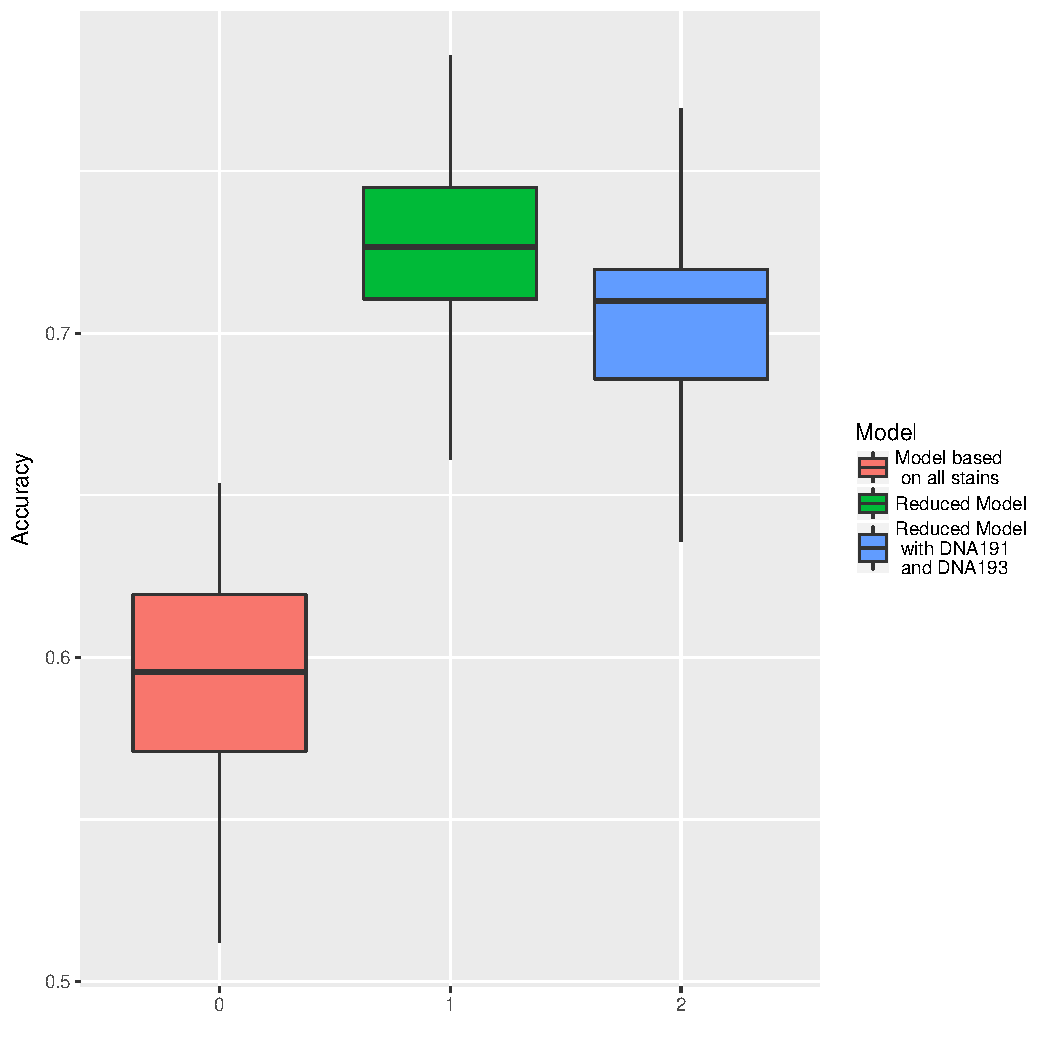
\includegraphics[width=\maxwidth]{figure/FigModelCrossVal1-1} \caption[Mean accuracy achieved during cross-validation]{Mean accuracy achieved during cross-validation. The model based on the step search with DNA193 removed does best.}\label{fig:FigModelCrossVal1}
\end{figure}


\end{knitrout}

\section{Further Refinement}
The model I get out of the \texttt{step()} optimisation still contains some covariates whose coefficients are not significant. Let's remove them and see what effect that has on the model.

Firstly, what are the coefficients and their p-values?
\begin{knitrout}
\definecolor{shadecolor}{rgb}{0.969, 0.969, 0.969}\color{fgcolor}\begin{kframe}
\begin{alltt}
\hlstd{pValVec} \hlkwb{=} \hlkwd{summary}\hlstd{(naiveStepSearch)}\hlopt{$}\hlstd{coefficients[,}\hlnum{4}\hlstd{]}
\hlstd{pValVec[}\hlkwd{order}\hlstd{(pValVec,}\hlkwc{decreasing}\hlstd{=T)]}
\end{alltt}
\begin{verbatim}
##          CD163           CD14            pS6           CD19        `PD-L2` 
##    0.331789897    0.124428814    0.109172121    0.087053506    0.084181459 
##           CD25            p21       Vimentin           CD8a           CD16 
##    0.073406710    0.061769923    0.049834705    0.046300187    0.031605949 
##          CD44s          FoxP3 `Beta-catenin`    (Intercept)         DNA191 
##    0.027242706    0.025420833    0.019722636    0.010703676    0.009830995 
##          CD152          CD134   `E-cadherin`           CD68          CD196 
##    0.002767454    0.002738525    0.001632426    0.001304554    0.001021551
\end{verbatim}
\end{kframe}
\end{knitrout}

This suggests removing CD163. CD163 is a monocyte/macrophage lineage marker, and as such seems to be the same as CD68. Is it co-linear with it?
\begin{knitrout}
\definecolor{shadecolor}{rgb}{0.969, 0.969, 0.969}\color{fgcolor}\begin{kframe}
\begin{alltt}
\hlstd{cd163Model} \hlkwb{=} \hlkwd{lm}\hlstd{(CD163}\hlopt{~}\hlstd{.,meanStainWide_Tranformed[,}\hlnum{2}\hlopt{:}\hlkwd{length}\hlstd{(meanStainWide_Tranformed)])}
\hlkwd{summary}\hlstd{(cd163Model)}
\end{alltt}
\begin{verbatim}
## 
## Call:
## lm(formula = CD163 ~ ., data = meanStainWide_Tranformed[, 2:length(meanStainWide_Tranformed)])
## 
## Residuals:
##     Min      1Q  Median      3Q     Max 
## -0.9732 -0.2434 -0.0421  0.1330  5.3980 
## 
## Coefficients:
##                  Estimate Std. Error t value Pr(>|t|)    
## (Intercept)    -3.101e-16  6.375e-02   0.000  1.00000    
## SrBCK           2.655e-01  2.023e-01   1.312  0.19295    
## RR101          -1.989e-01  1.454e+00  -0.137  0.89149    
## RR102           7.171e-03  1.427e+00   0.005  0.99600    
## AvantiLipid     1.732e-01  1.727e-01   1.003  0.31874    
## XeBCK          -3.371e-01  1.919e-01  -1.756  0.08270 .  
## CD196           5.325e-01  1.697e-01   3.138  0.00235 ** 
## CD19            1.626e-01  1.741e-01   0.934  0.35274    
## Vimentin        7.863e-02  1.160e-01   0.678  0.49976    
## CD20           -1.288e-02  1.085e-01  -0.119  0.90580    
## CD16            6.724e-01  1.620e-01   4.152 7.89e-05 ***
## CD25           -5.462e-01  1.989e-01  -2.746  0.00738 ** 
## p53             9.303e-02  7.666e-02   1.213  0.22835    
## CD134           6.682e-02  1.214e-01   0.550  0.58349    
## CD45            1.496e-01  1.508e-01   0.992  0.32428    
## CD44s          -1.213e-01  1.032e-01  -1.176  0.24303    
## CD14           -2.079e-01  1.704e-01  -1.220  0.22591    
## FoxP3          -4.377e-01  4.363e-01  -1.003  0.31873    
## CD4             3.101e-01  2.488e-01   1.246  0.21609    
## `E-cadherin`   -1.331e-01  1.428e-01  -0.932  0.35384    
## p21             1.639e-01  1.870e-01   0.877  0.38324    
## CD152          -5.954e-02  1.788e-01  -0.333  0.74003    
## CD8a           -4.756e-03  2.805e-01  -0.017  0.98651    
## CD11b          -2.448e-02  3.208e-01  -0.076  0.93936    
## `Beta-catenin`  1.026e-01  2.987e-01   0.344  0.73206    
## `B7-H4`         1.803e-02  1.485e-01   0.121  0.90369    
## Ki67            6.399e-02  1.365e-01   0.469  0.64045    
## CollagenI      -3.938e-02  1.191e-01  -0.331  0.74176    
## CD3            -2.004e-01  2.631e-01  -0.762  0.44830    
## CD68           -3.839e-01  5.144e-01  -0.746  0.45752    
## `PD-L2`        -2.218e-01  3.191e-01  -0.695  0.48898    
## `B7-H3`         5.040e-01  2.307e-01   2.184  0.03172 *  
## `HLA-DR`        2.736e-01  6.188e-01   0.442  0.65949    
## pS6            -1.481e-01  1.641e-01  -0.903  0.36918    
## HistoneH3      -9.189e-02  4.839e-01  -0.190  0.84985    
## DNA191         -5.682e+00  3.552e+00  -1.600  0.11345    
## DNA193          5.902e+00  3.576e+00   1.651  0.10255    
## ---
## Signif. codes:  0 '***' 0.001 '**' 0.01 '*' 0.05 '.' 0.1 ' ' 1
## 
## Residual standard error: 0.7012 on 84 degrees of freedom
## Multiple R-squared:  0.6558,	Adjusted R-squared:  0.5083 
## F-statistic: 4.446 on 36 and 84 DF,  p-value: 9.394e-09
\end{verbatim}
\end{kframe}
\end{knitrout}
Interestingly not. But it is strongly correlated with CD16, a generic immune marker.

Let's drop it.
\begin{knitrout}
\definecolor{shadecolor}{rgb}{0.969, 0.969, 0.969}\color{fgcolor}\begin{kframe}
\begin{alltt}
\hlstd{minimalModel} \hlkwb{=} \hlkwd{update}\hlstd{(naiveStepSearch,.}\hlopt{~}\hlstd{.}\hlopt{-}\hlstd{CD163)}
\hlkwd{summary}\hlstd{(minimalModel)}
\end{alltt}
\begin{verbatim}
## 
## Call:
## glm(formula = PtSnty ~ CD196 + CD19 + Vimentin + CD16 + CD25 + 
##     CD134 + CD44s + CD14 + FoxP3 + `E-cadherin` + p21 + CD152 + 
##     CD8a + `Beta-catenin` + CD68 + `PD-L2` + pS6 + DNA191, family = binomial(link = "logit"), 
##     data = meanStainWide_LessCorr)
## 
## Deviance Residuals: 
##     Min       1Q   Median       3Q      Max  
## -2.8758  -0.4584   0.2269   0.6605   1.5814  
## 
## Coefficients:
##                Estimate Std. Error z value Pr(>|z|)    
## (Intercept)      0.8492     0.3224   2.634 0.008442 ** 
## CD196            2.6966     0.8070   3.342 0.000833 ***
## CD19             2.6623     1.5772   1.688 0.091423 .  
## Vimentin        -0.6926     0.3827  -1.810 0.070310 .  
## CD16            -1.4582     0.7844  -1.859 0.063007 .  
## CD25            -3.8760     2.1816  -1.777 0.075612 .  
## CD134           -1.7148     0.5893  -2.910 0.003617 ** 
## CD44s            0.8567     0.4151   2.064 0.039014 *  
## CD14             0.9287     0.6473   1.435 0.151355    
## FoxP3           -1.9957     1.0044  -1.987 0.046937 *  
## `E-cadherin`     2.1653     0.7108   3.046 0.002319 ** 
## p21              1.8358     1.0024   1.831 0.067058 .  
## CD152           -2.1043     0.7118  -2.956 0.003112 ** 
## CD8a            -2.1134     1.0405  -2.031 0.042238 *  
## `Beta-catenin`  -3.1216     1.3518  -2.309 0.020933 *  
## CD68             4.0451     1.3070   3.095 0.001969 ** 
## `PD-L2`          2.1657     1.2126   1.786 0.074106 .  
## pS6             -0.8631     0.5722  -1.508 0.131455    
## DNA191           1.0514     0.4273   2.461 0.013874 *  
## ---
## Signif. codes:  0 '***' 0.001 '**' 0.01 '*' 0.05 '.' 0.1 ' ' 1
## 
## (Dispersion parameter for binomial family taken to be 1)
## 
##     Null deviance: 161.666  on 120  degrees of freedom
## Residual deviance:  95.512  on 102  degrees of freedom
## AIC: 133.51
## 
## Number of Fisher Scoring iterations: 7
\end{verbatim}
\end{kframe}
\end{knitrout}

The next one to drop seems to be CD14 (again a macrophage marker). Let's drop this:
\begin{knitrout}
\definecolor{shadecolor}{rgb}{0.969, 0.969, 0.969}\color{fgcolor}\begin{kframe}
\begin{alltt}
\hlstd{minimalModel} \hlkwb{=} \hlkwd{update}\hlstd{(minimalModel,.}\hlopt{~}\hlstd{.}\hlopt{-}\hlstd{CD14)}
\hlkwd{summary}\hlstd{(minimalModel)}
\end{alltt}
\begin{verbatim}
## 
## Call:
## glm(formula = PtSnty ~ CD196 + CD19 + Vimentin + CD16 + CD25 + 
##     CD134 + CD44s + FoxP3 + `E-cadherin` + p21 + CD152 + CD8a + 
##     `Beta-catenin` + CD68 + `PD-L2` + pS6 + DNA191, family = binomial(link = "logit"), 
##     data = meanStainWide_LessCorr)
## 
## Deviance Residuals: 
##     Min       1Q   Median       3Q      Max  
## -2.8646  -0.5166   0.1700   0.6888   1.9140  
## 
## Coefficients:
##                Estimate Std. Error z value Pr(>|z|)    
## (Intercept)      0.8884     0.3186   2.789 0.005294 ** 
## CD196            2.6207     0.7828   3.348 0.000814 ***
## CD19             2.7327     1.6502   1.656 0.097723 .  
## Vimentin        -0.7179     0.3761  -1.909 0.056265 .  
## CD16            -1.0153     0.5896  -1.722 0.085090 .  
## CD25            -3.9669     2.2723  -1.746 0.080852 .  
## CD134           -1.7024     0.5682  -2.996 0.002737 ** 
## CD44s            0.9085     0.4059   2.238 0.025194 *  
## FoxP3           -2.0848     0.9954  -2.094 0.036228 *  
## `E-cadherin`     2.0166     0.6742   2.991 0.002778 ** 
## p21              1.6047     0.8804   1.823 0.068350 .  
## CD152           -1.8171     0.6102  -2.978 0.002904 ** 
## CD8a            -1.1990     0.8200  -1.462 0.143693    
## `Beta-catenin`  -2.4310     1.1881  -2.046 0.040746 *  
## CD68             3.9591     1.2234   3.236 0.001212 ** 
## `PD-L2`          1.3020     0.9792   1.330 0.183637    
## pS6             -1.0540     0.5507  -1.914 0.055643 .  
## DNA191           1.1815     0.4212   2.805 0.005031 ** 
## ---
## Signif. codes:  0 '***' 0.001 '**' 0.01 '*' 0.05 '.' 0.1 ' ' 1
## 
## (Dispersion parameter for binomial family taken to be 1)
## 
##     Null deviance: 161.666  on 120  degrees of freedom
## Residual deviance:  97.571  on 103  degrees of freedom
## AIC: 133.57
## 
## Number of Fisher Scoring iterations: 7
\end{verbatim}
\end{kframe}
\end{knitrout}

The next one to drop is PD-L2:
\begin{knitrout}
\definecolor{shadecolor}{rgb}{0.969, 0.969, 0.969}\color{fgcolor}\begin{kframe}
\begin{alltt}
\hlstd{minimalModel} \hlkwb{=} \hlkwd{update}\hlstd{(minimalModel,.}\hlopt{~}\hlstd{.}\hlopt{-}\hlstd{`PD-L2`)}
\hlkwd{summary}\hlstd{(minimalModel)}
\end{alltt}
\begin{verbatim}
## 
## Call:
## glm(formula = PtSnty ~ CD196 + CD19 + Vimentin + CD16 + CD25 + 
##     CD134 + CD44s + FoxP3 + `E-cadherin` + p21 + CD152 + CD8a + 
##     `Beta-catenin` + CD68 + pS6 + DNA191, family = binomial(link = "logit"), 
##     data = meanStainWide_LessCorr)
## 
## Deviance Residuals: 
##     Min       1Q   Median       3Q      Max  
## -2.8314  -0.6047   0.1908   0.6836   1.7648  
## 
## Coefficients:
##                Estimate Std. Error z value Pr(>|z|)    
## (Intercept)      0.8582     0.3160   2.716 0.006610 ** 
## CD196            2.5588     0.7649   3.345 0.000822 ***
## CD19             2.7742     1.6485   1.683 0.092411 .  
## Vimentin        -0.7674     0.3671  -2.090 0.036574 *  
## CD16            -1.0619     0.6424  -1.653 0.098307 .  
## CD25            -3.9443     2.2525  -1.751 0.079924 .  
## CD134           -1.9699     0.5514  -3.572 0.000354 ***
## CD44s            0.7679     0.3706   2.072 0.038284 *  
## FoxP3           -2.2300     0.9614  -2.320 0.020359 *  
## `E-cadherin`     1.9907     0.6754   2.948 0.003203 ** 
## p21              1.6060     0.7715   2.082 0.037374 *  
## CD152           -1.4403     0.5194  -2.773 0.005554 ** 
## CD8a            -0.7888     0.7083  -1.114 0.265378    
## `Beta-catenin`  -1.3989     0.8107  -1.726 0.084428 .  
## CD68             3.8826     1.2117   3.204 0.001354 ** 
## pS6             -1.1122     0.5385  -2.065 0.038892 *  
## DNA191           1.2522     0.4200   2.982 0.002868 ** 
## ---
## Signif. codes:  0 '***' 0.001 '**' 0.01 '*' 0.05 '.' 0.1 ' ' 1
## 
## (Dispersion parameter for binomial family taken to be 1)
## 
##     Null deviance: 161.666  on 120  degrees of freedom
## Residual deviance:  99.379  on 104  degrees of freedom
## AIC: 133.38
## 
## Number of Fisher Scoring iterations: 7
\end{verbatim}
\end{kframe}
\end{knitrout}

And then CD8a (cytotoxic T-cells). Note: the AIC has remained almost unchanged up to now (Before: 133.2143738, Now: 133.3793751)
\begin{knitrout}
\definecolor{shadecolor}{rgb}{0.969, 0.969, 0.969}\color{fgcolor}\begin{kframe}
\begin{alltt}
\hlstd{minimalModel} \hlkwb{=} \hlkwd{update}\hlstd{(minimalModel,.}\hlopt{~}\hlstd{.}\hlopt{-}\hlstd{`CD8a`)}
\hlkwd{summary}\hlstd{(minimalModel)}
\end{alltt}
\begin{verbatim}
## 
## Call:
## glm(formula = PtSnty ~ CD196 + CD19 + Vimentin + CD16 + CD25 + 
##     CD134 + CD44s + FoxP3 + `E-cadherin` + p21 + CD152 + `Beta-catenin` + 
##     CD68 + pS6 + DNA191, family = binomial(link = "logit"), data = meanStainWide_LessCorr)
## 
## Deviance Residuals: 
##     Min       1Q   Median       3Q      Max  
## -2.8602  -0.6006   0.1554   0.7108   1.7510  
## 
## Coefficients:
##                Estimate Std. Error z value Pr(>|z|)    
## (Intercept)      0.9039     0.3127   2.891 0.003845 ** 
## CD196            2.3658     0.7127   3.320 0.000902 ***
## CD19             2.6282     1.5051   1.746 0.080770 .  
## Vimentin        -0.6319     0.3356  -1.883 0.059712 .  
## CD16            -1.0518     0.6358  -1.654 0.098070 .  
## CD25            -3.5926     2.0346  -1.766 0.077430 .  
## CD134           -1.8467     0.5144  -3.590 0.000330 ***
## CD44s            0.7111     0.3565   1.995 0.046059 *  
## FoxP3           -2.1527     0.9503  -2.265 0.023503 *  
## `E-cadherin`     1.9864     0.6652   2.986 0.002823 ** 
## p21              1.5668     0.7958   1.969 0.048968 *  
## CD152           -1.4808     0.5181  -2.858 0.004262 ** 
## `Beta-catenin`  -1.5880     0.8078  -1.966 0.049303 *  
## CD68             3.2587     1.0426   3.126 0.001774 ** 
## pS6             -0.9890     0.4977  -1.987 0.046894 *  
## DNA191           1.2208     0.4092   2.984 0.002849 ** 
## ---
## Signif. codes:  0 '***' 0.001 '**' 0.01 '*' 0.05 '.' 0.1 ' ' 1
## 
## (Dispersion parameter for binomial family taken to be 1)
## 
##     Null deviance: 161.67  on 120  degrees of freedom
## Residual deviance: 100.49  on 105  degrees of freedom
## AIC: 132.49
## 
## Number of Fisher Scoring iterations: 7
\end{verbatim}
\end{kframe}
\end{knitrout}

Now the p-values are all below 0.1 and the AIC is also lower than any other model so far (AIC = 132.4854583). How are the VIFs?

\begin{knitrout}
\definecolor{shadecolor}{rgb}{0.969, 0.969, 0.969}\color{fgcolor}\begin{kframe}
\begin{alltt}
\hlstd{vifVec} \hlkwb{=} \hlkwd{vif}\hlstd{(minimalModel)}
\hlstd{vifVec[}\hlkwd{order}\hlstd{(vifVec,}\hlkwc{decreasing}\hlstd{=T)]}
\end{alltt}
\begin{verbatim}
##           CD25           CD19           CD68          FoxP3 `Beta-catenin` 
##      39.162802      37.143459      14.129555      13.790241      11.196649 
##            p21          CD196   `E-cadherin`          CD152            pS6 
##       8.157373       5.952418       5.782691       4.999685       4.683451 
##           CD16          CD134         DNA191          CD44s       Vimentin 
##       4.447130       3.577718       3.073502       1.877000       1.781078
\end{verbatim}
\end{kframe}
\end{knitrout}

Mhm, still not great. How does the plot look like?
\begin{knitrout}
\definecolor{shadecolor}{rgb}{0.969, 0.969, 0.969}\color{fgcolor}\begin{kframe}
\begin{alltt}
\hlkwd{PlotCoefficients}\hlstd{(minimalModel,}\hlkwc{yLim}\hlstd{=}\hlkwd{c}\hlstd{(}\hlopt{-}\hlnum{30}\hlstd{,}\hlnum{30}\hlstd{),}\hlkwc{yPos}\hlstd{=}\hlnum{22}\hlstd{,}\hlkwc{errBarWidth}\hlstd{=}\hlnum{.4}\hlstd{)}
\end{alltt}
\end{kframe}\begin{figure}[h]
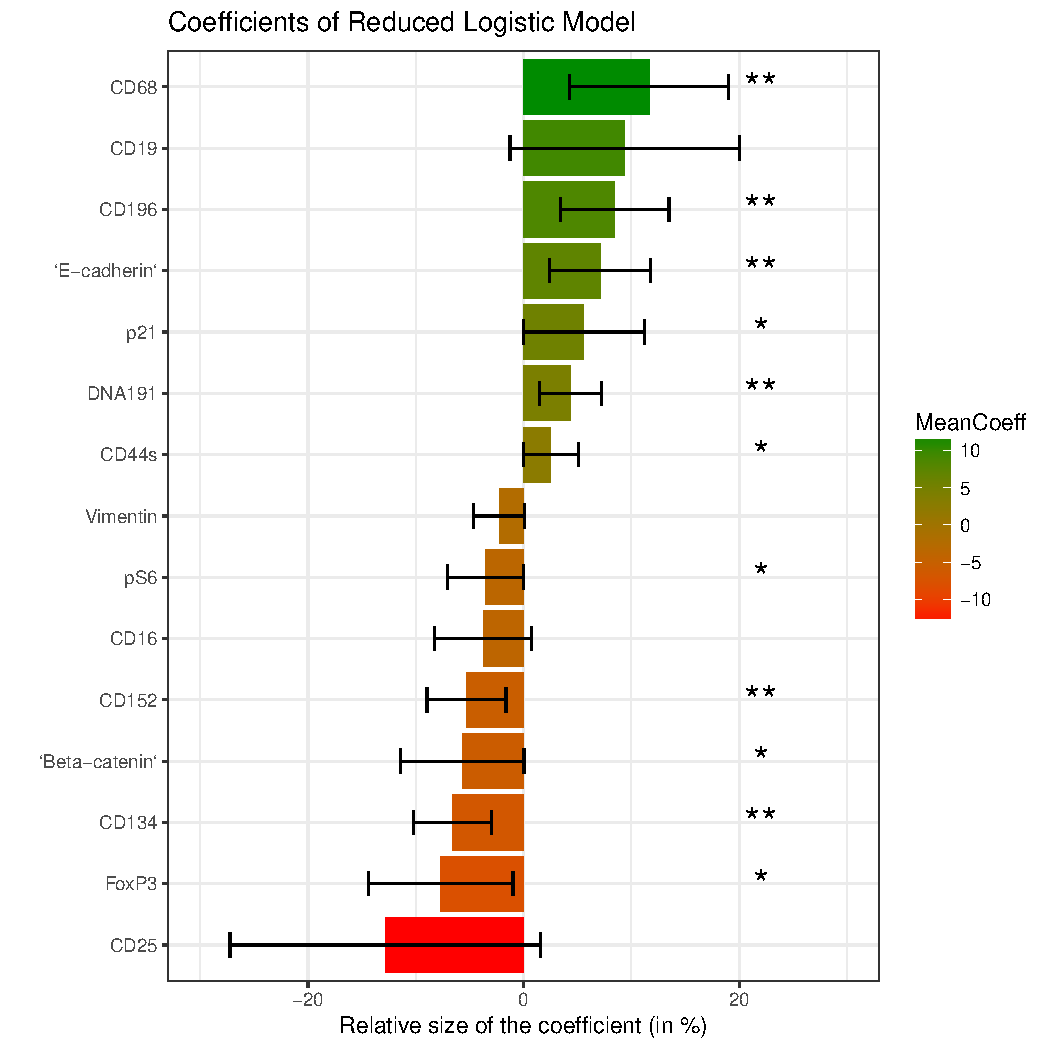
\includegraphics[width=\maxwidth]{figure/Fig_minModCoeff-1} \caption[Importance of the different stains according to the reduced logistic model]{Importance of the different stains according to the reduced logistic model. Asterisk indicates level of statistical support for non-zero contribution from this stain (T-test: *p$<$0.05,**p$<$0.01).}\label{fig:Fig_minModCoeff}
\end{figure}


\end{knitrout}

How is it's performance?
\begin{knitrout}
\definecolor{shadecolor}{rgb}{0.969, 0.969, 0.969}\color{fgcolor}\begin{kframe}
\begin{alltt}
\hlstd{nIter} \hlkwb{=} \hlnum{100}
\hlstd{nFolds} \hlkwb{=} \hlnum{5}

\hlcom{# Do the cross validation}
\hlstd{minModAccVec} \hlkwb{=} \hlkwd{LogisticCrossVal}\hlstd{(nIter,nFolds,minimalModel}\hlopt{$}\hlstd{formula,}
                                \hlstd{meanStainWide_Tranformed)}

\hlcom{# Plot the results}
\hlstd{xValidResult} \hlkwb{=} \hlkwd{data.frame}\hlstd{(}\hlkwc{Accuracy}\hlstd{=}\hlkwd{c}\hlstd{(fullModAccVec,redModAccVec,}
                                     \hlstd{redModAccVec_BothDNAs,minModAccVec),}
                          \hlkwc{Model}\hlstd{=}\hlkwd{as.factor}\hlstd{(}\hlkwd{c}\hlstd{(}\hlkwd{rep}\hlstd{(}\hlnum{0}\hlstd{,nIter),}\hlkwd{rep}\hlstd{(}\hlnum{1}\hlstd{,nIter),}
                                            \hlkwd{rep}\hlstd{(}\hlnum{2}\hlstd{,nIter),}\hlkwd{rep}\hlstd{(}\hlnum{3}\hlstd{,nIter))))}
\hlkwd{ggplot}\hlstd{(xValidResult,}\hlkwd{aes}\hlstd{(}\hlkwc{x}\hlstd{=Model,}\hlkwc{y}\hlstd{=Accuracy,}\hlkwc{fill}\hlstd{=Model))} \hlopt{+}
  \hlkwd{geom_boxplot}\hlstd{()} \hlopt{+}
  \hlkwd{xlab}\hlstd{(}\hlstr{""}\hlstd{)} \hlopt{+}
  \hlkwd{scale_fill_discrete}\hlstd{(}\hlkwc{breaks}\hlstd{=}\hlkwd{seq}\hlstd{(}\hlnum{0}\hlstd{,}\hlnum{3}\hlstd{),}\hlkwc{labels}\hlstd{=}\hlkwd{c}\hlstd{(}\hlstr{"Model based\textbackslash{}n on all stains"}\hlstd{,}
                                               \hlstr{"Reduced Model"}\hlstd{,}
                                               \hlstr{"Reduced Model\textbackslash{}n with DNA191\textbackslash{}n and DNA193"}\hlstd{,}
                                               \hlstr{"Minimal Model"}\hlstd{))}
\end{alltt}
\end{kframe}\begin{figure}[h]
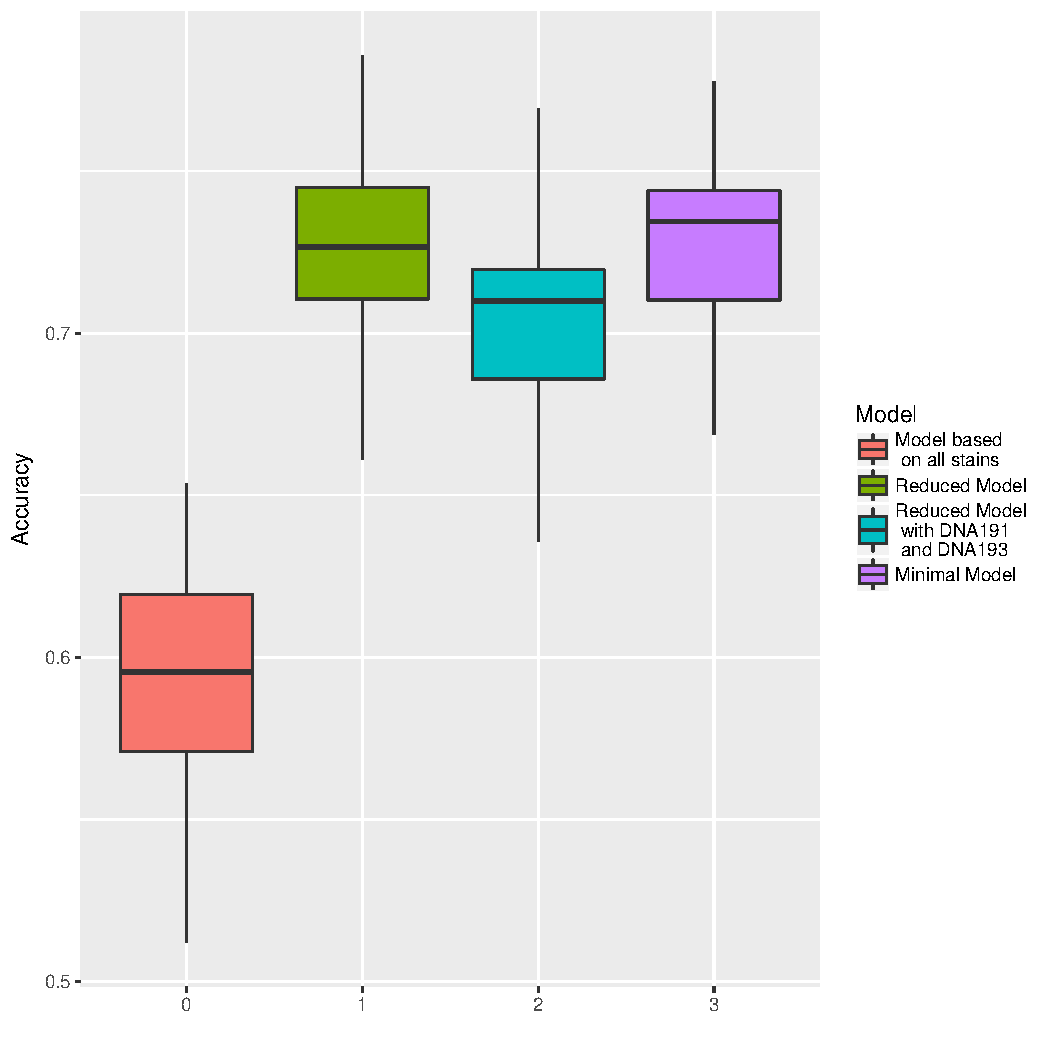
\includegraphics[width=\maxwidth]{figure/FigModelCrossVal2-1} \caption[Mean accuracy achieved during cross-validation]{Mean accuracy achieved during cross-validation. The minimal model still does as well as before removing the extra stains.}\label{fig:FigModelCrossVal2}
\end{figure}


\end{knitrout}
So, it has been able to maintain its performance!

\section{Biological Interpretation}
Now that we have reduced the data to a small number of stains (16) let's see what the results suggest. What is the biological meaning of our results?
\begin{knitrout}
\definecolor{shadecolor}{rgb}{0.969, 0.969, 0.969}\color{fgcolor}\begin{kframe}
\begin{alltt}
\hlstd{p} \hlkwb{=} \hlkwd{PlotCoefficients}\hlstd{(minimalModel,}\hlkwc{yLim}\hlstd{=}\hlkwd{c}\hlstd{(}\hlopt{-}\hlnum{50}\hlstd{,}\hlnum{50}\hlstd{),}\hlkwc{yPos}\hlstd{=}\hlnum{22}\hlstd{,}\hlkwc{errBarWidth}\hlstd{=}\hlnum{.4}\hlstd{)}

\hlcom{# Annotate the markers}
\hlstd{yPos} \hlkwb{=} \hlnum{37}
\hlstd{tSize} \hlkwb{=} \hlnum{2.5}
\hlcom{# Positive}
\hlstd{p} \hlkwb{=} \hlstd{p} \hlopt{+} \hlkwd{annotate}\hlstd{(}\hlstr{"text"}\hlstd{,} \hlkwc{x} \hlstd{=} \hlstr{"CD68"}\hlstd{,} \hlkwc{y} \hlstd{= yPos,}
                       \hlkwc{label} \hlstd{=} \hlstr{"Monocytes/\textbackslash{}n Macrophages"}\hlstd{,} \hlkwc{size} \hlstd{= tSize)}
\hlstd{p} \hlkwb{=} \hlstd{p} \hlopt{+} \hlkwd{annotate}\hlstd{(}\hlstr{"text"}\hlstd{,} \hlkwc{x} \hlstd{=} \hlstr{"CD19"}\hlstd{,} \hlkwc{y} \hlstd{= yPos,}
                       \hlkwc{label} \hlstd{=} \hlstr{"B-Cells"}\hlstd{,} \hlkwc{size} \hlstd{= tSize)}
\hlstd{p} \hlkwb{=} \hlstd{p} \hlopt{+} \hlkwd{annotate}\hlstd{(}\hlstr{"text"}\hlstd{,} \hlkwc{x} \hlstd{=} \hlstr{"CD196"}\hlstd{,} \hlkwc{y} \hlstd{= yPos,}
                       \hlkwc{label} \hlstd{=} \hlstr{"Immature Dendritic Cells/\textbackslash{}n Memory T-Cells"}\hlstd{,} \hlkwc{size} \hlstd{= tSize)}
\hlstd{p} \hlkwb{=} \hlstd{p} \hlopt{+} \hlkwd{annotate}\hlstd{(}\hlstr{"text"}\hlstd{,} \hlkwc{x} \hlstd{=} \hlstr{"`E-cadherin`"}\hlstd{,} \hlkwc{y} \hlstd{= yPos,}
                       \hlkwc{label} \hlstd{=} \hlstr{"Epithelial Phenotype"}\hlstd{,} \hlkwc{size} \hlstd{= tSize)}
\hlstd{p} \hlkwb{=} \hlstd{p} \hlopt{+} \hlkwd{annotate}\hlstd{(}\hlstr{"text"}\hlstd{,} \hlkwc{x} \hlstd{=} \hlstr{"p21"}\hlstd{,} \hlkwc{y} \hlstd{= yPos,}
                       \hlkwc{label} \hlstd{=} \hlstr{"Cell Cycle Inhibitor"}\hlstd{,} \hlkwc{size} \hlstd{= tSize)}
\hlstd{p} \hlkwb{=} \hlstd{p} \hlopt{+} \hlkwd{annotate}\hlstd{(}\hlstr{"text"}\hlstd{,} \hlkwc{x} \hlstd{=} \hlstr{"DNA191"}\hlstd{,} \hlkwc{y} \hlstd{= yPos,}
                       \hlkwc{label} \hlstd{=} \hlstr{"NA"}\hlstd{,} \hlkwc{size} \hlstd{= tSize)}
\hlstd{p} \hlkwb{=} \hlstd{p} \hlopt{+} \hlkwd{annotate}\hlstd{(}\hlstr{"text"}\hlstd{,} \hlkwc{x} \hlstd{=} \hlstr{"DNA191"}\hlstd{,} \hlkwc{y} \hlstd{= yPos,}
                       \hlkwc{label} \hlstd{=} \hlstr{"NA"}\hlstd{,} \hlkwc{size} \hlstd{= tSize)}
\hlstd{p} \hlkwb{=} \hlstd{p} \hlopt{+} \hlkwd{annotate}\hlstd{(}\hlstr{"text"}\hlstd{,} \hlkwc{x} \hlstd{=} \hlstr{"CD44s"}\hlstd{,} \hlkwc{y} \hlstd{= yPos,}
                       \hlkwc{label} \hlstd{=} \hlstr{"Cell-Cell Interaction"}\hlstd{,} \hlkwc{size} \hlstd{= tSize)}
\hlstd{p} \hlkwb{=} \hlstd{p} \hlopt{+} \hlkwd{geom_rect}\hlstd{(}\hlkwd{aes}\hlstd{(}\hlkwc{xmin} \hlstd{=} \hlstr{"Vimentin"}\hlstd{,} \hlkwc{xmax} \hlstd{=} \hlnum{16.5}\hlstd{,} \hlkwc{ymin} \hlstd{=} \hlnum{25}\hlstd{,} \hlkwc{ymax} \hlstd{=} \hlnum{50}\hlstd{),}
               \hlkwc{fill} \hlstd{=} \hlstr{"transparent"}\hlstd{,} \hlkwc{color} \hlstd{=} \hlstr{"green4"}\hlstd{,} \hlkwc{size} \hlstd{=} \hlnum{1.5}\hlstd{)}

\hlcom{# Negative}
\hlstd{yPos} \hlkwb{=} \hlopt{-}\hlnum{37}
\hlstd{p} \hlkwb{=} \hlstd{p} \hlopt{+} \hlkwd{annotate}\hlstd{(}\hlstr{"text"}\hlstd{,} \hlkwc{x} \hlstd{=} \hlstr{"Vimentin"}\hlstd{,} \hlkwc{y} \hlstd{= yPos,}
                       \hlkwc{label} \hlstd{=} \hlstr{"Mesenchymal Phenotype"}\hlstd{,} \hlkwc{size} \hlstd{= tSize)}
\hlstd{p} \hlkwb{=} \hlstd{p} \hlopt{+} \hlkwd{annotate}\hlstd{(}\hlstr{"text"}\hlstd{,} \hlkwc{x} \hlstd{=} \hlstr{"pS6"}\hlstd{,} \hlkwc{y} \hlstd{= yPos,}
                       \hlkwc{label} \hlstd{=} \hlstr{"Increased Translation"}\hlstd{,} \hlkwc{size} \hlstd{= tSize)}
\hlstd{p} \hlkwb{=} \hlstd{p} \hlopt{+} \hlkwd{annotate}\hlstd{(}\hlstr{"text"}\hlstd{,} \hlkwc{x} \hlstd{=} \hlstr{"CD16"}\hlstd{,} \hlkwc{y} \hlstd{= yPos,}
                       \hlkwc{label} \hlstd{=} \hlstr{"Monocytes/\textbackslash{}n Macrophages/\textbackslash{}n NK Cells"}\hlstd{,} \hlkwc{size} \hlstd{= tSize)}
\hlstd{p} \hlkwb{=} \hlstd{p} \hlopt{+} \hlkwd{annotate}\hlstd{(}\hlstr{"text"}\hlstd{,} \hlkwc{x} \hlstd{=} \hlstr{"CD152"}\hlstd{,} \hlkwc{y} \hlstd{= yPos,}
                       \hlkwc{label} \hlstd{=} \hlstr{"Checkpoint Inhibitor"}\hlstd{,} \hlkwc{size} \hlstd{= tSize)}
\hlstd{p} \hlkwb{=} \hlstd{p} \hlopt{+} \hlkwd{annotate}\hlstd{(}\hlstr{"text"}\hlstd{,} \hlkwc{x} \hlstd{=} \hlstr{"`Beta-catenin`"}\hlstd{,} \hlkwc{y} \hlstd{= yPos,}
                       \hlkwc{label} \hlstd{=} \hlstr{"Proto-Oncogene\textbackslash{}n Wnt Pathway"}\hlstd{,} \hlkwc{size} \hlstd{= tSize)}
\hlstd{p} \hlkwb{=} \hlstd{p} \hlopt{+} \hlkwd{annotate}\hlstd{(}\hlstr{"text"}\hlstd{,} \hlkwc{x} \hlstd{=} \hlstr{"CD134"}\hlstd{,} \hlkwc{y} \hlstd{= yPos,}
                       \hlkwc{label} \hlstd{=} \hlstr{"T-Cell Activation\textbackslash{}n Survival"}\hlstd{,} \hlkwc{size} \hlstd{= tSize)}
\hlstd{p} \hlkwb{=} \hlstd{p} \hlopt{+} \hlkwd{annotate}\hlstd{(}\hlstr{"text"}\hlstd{,} \hlkwc{x} \hlstd{=} \hlstr{"FoxP3"}\hlstd{,} \hlkwc{y} \hlstd{= yPos,}
                       \hlkwc{label} \hlstd{=} \hlstr{"Regulatory T-Cells"}\hlstd{,} \hlkwc{size} \hlstd{= tSize)}
\hlstd{p} \hlkwb{=} \hlstd{p} \hlopt{+} \hlkwd{annotate}\hlstd{(}\hlstr{"text"}\hlstd{,} \hlkwc{x} \hlstd{=} \hlstr{"CD25"}\hlstd{,} \hlkwc{y} \hlstd{= yPos,}
                       \hlkwc{label} \hlstd{=} \hlstr{"Activated T- and B-Cells"}\hlstd{,} \hlkwc{size} \hlstd{= tSize)}
\hlstd{p} \hlkwb{=} \hlstd{p} \hlopt{+} \hlkwd{geom_rect}\hlstd{(}\hlkwd{aes}\hlstd{(}\hlkwc{xmin} \hlstd{=} \hlnum{0}\hlstd{,} \hlkwc{xmax} \hlstd{=} \hlstr{"CD44s"}\hlstd{,} \hlkwc{ymin} \hlstd{=} \hlopt{-}\hlnum{25}\hlstd{,} \hlkwc{ymax} \hlstd{=} \hlopt{-}\hlnum{50}\hlstd{),}
               \hlkwc{fill} \hlstd{=} \hlstr{"transparent"}\hlstd{,} \hlkwc{color} \hlstd{=} \hlstr{"red"}\hlstd{,} \hlkwc{size} \hlstd{=} \hlnum{1.5}\hlstd{)}

\hlstd{p}
\end{alltt}
\end{kframe}\begin{figure}[h]
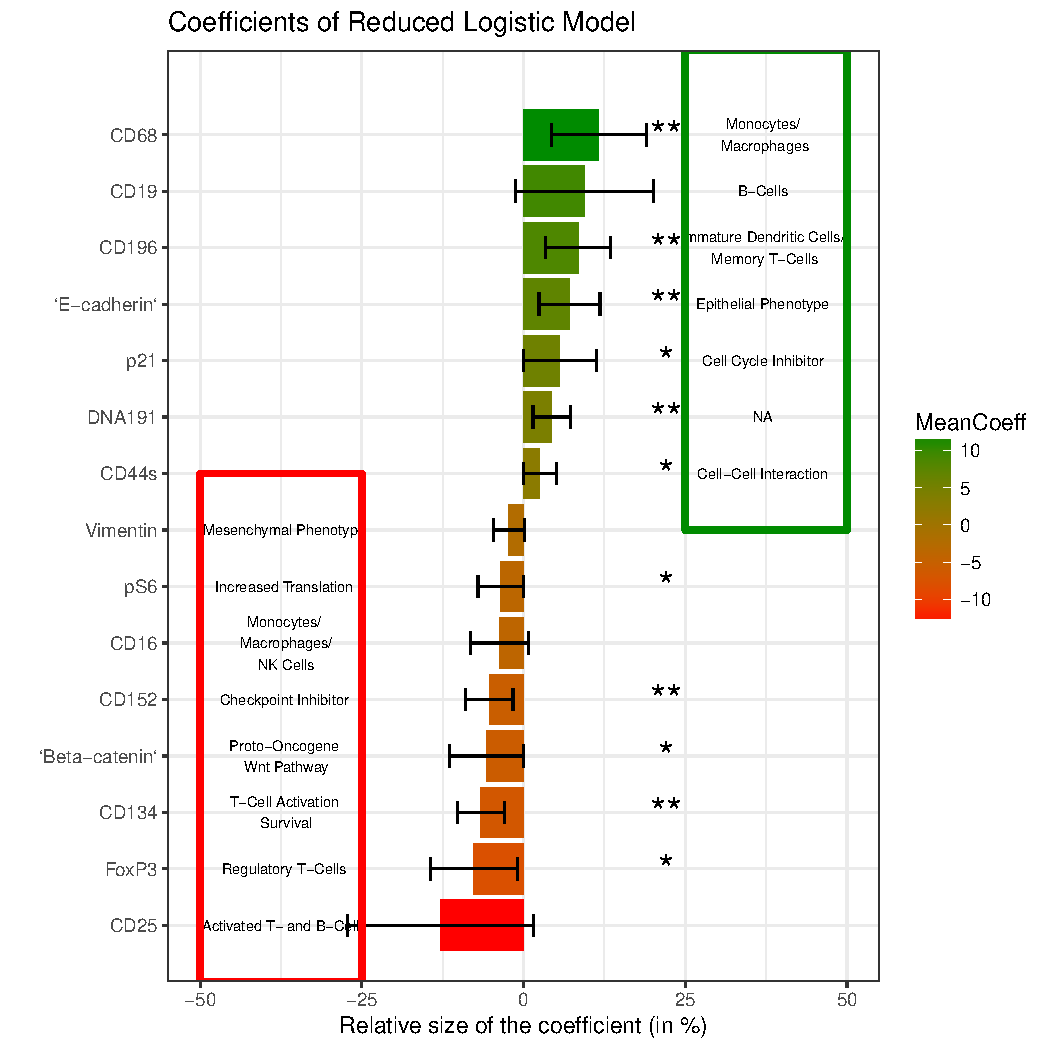
\includegraphics[width=\maxwidth]{figure/Fig_minModCoeff_Annot-1} \caption[Importance of the different stains according to the reduced logistic model]{Importance of the different stains according to the reduced logistic model. Asterisk indicates level of statistical support for non-zero contribution from this stain (T-test: *p$<$0.05,**p$<$0.01).}\label{fig:Fig_minModCoeff_Annot}
\end{figure}


\end{knitrout}

A lot of the correlation make biological sense (e.g. more mesenchymal phenotypes correlated with worse prognosis). When looking some of these markers up on wikipedia they all have the corresponding correlation with cancer.

Two are interesting:
CD44 can be both pro and anti cancer, depending on post-translational modifications/splicing (i.e. context). For ovarian, however, CD44 has been correlated in the past with good outcome ( Sillanpaa S, Anttila MA, Voutilainen K, Tammi RH, Tammi MI, Saarikoski SV, Kosma VM (Nov 2003). "CD44 expression indicates favorable prognosis in epithelial ovarian cancer". Clinical Cancer Research. 9 (14): 5318–24. PMID 14614016.). It's a hialuronic acid receptor.

CD134 is associated with longer t-cell survival. Similarly, FoxP3 indicates activated T-reg cells. Maybe we have protection from T-cells here?

\section{A Model on De-Correlated Data}
The model at this point still has very high VIFs which means there is still a lot of co-linearity. Also the errors on for example CD25 are very high, so there seems to be some kind of conflicting signal. Let's try to reduce the VIF to say 10 or 20 before doing model selection, so that the coefficient estimates (which model selection relies on!) are more reliable.

Below I define a set of functions that will de-correlate the data (\texttt{DecorrelateVariables()}) and do a stepping search on it that does both stepping (to minimise AIC) and dropping the variable with the highest VIF (to further reduce the VIFs).
\begin{knitrout}
\definecolor{shadecolor}{rgb}{0.969, 0.969, 0.969}\color{fgcolor}\begin{kframe}
\begin{alltt}
\hlcom{# Function to decorrelate the variables in an R regression model (of class lm or glm).}
\hlcom{# It drops the variable with the highest VIF until all VIFs are below targetVIF. VIF is a}
\hlcom{# measure of how well one variable can be expressed as a linear combination of the others.}
\hlstd{DecorrelateVariables} \hlkwb{=} \hlkwa{function}\hlstd{(}\hlkwc{model}\hlstd{,}\hlkwc{targetVIF}\hlstd{,}\hlkwc{verbose}\hlstd{=T) \{}
  \hlkwd{library}\hlstd{(car)}
  \hlkwa{repeat}\hlstd{\{}
    \hlcom{# Identify the variable with the maximum VIF }
    \hlstd{vifVec} \hlkwb{=} \hlkwd{vif}\hlstd{(model)}
    \hlstd{maxVIF} \hlkwb{=} \hlkwd{max}\hlstd{(vifVec)}
    \hlcom{# vif() output changes if there are factor variables in the model.}
    \hlcom{# Adjust for this.}
    \hlkwa{if}\hlstd{(}\hlkwd{is.null}\hlstd{(}\hlkwd{dim}\hlstd{(vifVec))) \{} \hlcom{# No factor}
      \hlstd{varToDrop} \hlkwb{=} \hlkwd{names}\hlstd{(vifVec)[}\hlkwd{which.max}\hlstd{(vifVec)]}
    \hlstd{\}} \hlkwa{else}\hlstd{\{} \hlcom{# Factor}
      \hlstd{varToDrop} \hlkwb{=} \hlkwd{names}\hlstd{(vifVec[,}\hlnum{1}\hlstd{])[}\hlkwd{which.max}\hlstd{(vifVec[,}\hlnum{1}\hlstd{])]}
    \hlstd{\}}

    \hlcom{# If the maximum VIF is below the target stop}
    \hlkwa{if} \hlstd{(maxVIF}\hlopt{<=}\hlstd{targetVIF)\{}
      \hlkwa{break}
    \hlstd{\}} \hlkwa{else} \hlstd{\{} \hlcom{# Else, drop that variable}
      \hlstd{model} \hlkwb{=} \hlkwd{update}\hlstd{(model,}\hlkwd{paste0}\hlstd{(}\hlstr{".~.-"}\hlstd{,varToDrop))}
      \hlkwa{if}\hlstd{(verbose) \{}\hlkwd{print}\hlstd{(}\hlkwd{paste0}\hlstd{(}\hlstr{"Dropping "}\hlstd{,varToDrop,}\hlstr{" with VIF "}\hlstd{,maxVIF))\}}
    \hlstd{\}}
  \hlstd{\}}
  \hlkwd{return}\hlstd{(model)}
\hlstd{\}}
\hlcom{# Function to compute the accuracy of the model in predicting the provided input variables}
\hlstd{LmAccuracy} \hlkwb{=} \hlkwa{function}\hlstd{(}\hlkwc{model}\hlstd{,}\hlkwc{classifier}\hlstd{=F) \{}
  \hlkwa{if}\hlstd{(classifier) \{}
     \hlstd{accuracy} \hlkwb{=} \hlkwd{mean}\hlstd{(}\hlkwd{ifelse}\hlstd{(model}\hlopt{$}\hlstd{fitted.values}\hlopt{>}\hlnum{0.5}\hlstd{,}\hlnum{1}\hlstd{,}\hlnum{0}\hlstd{)}\hlopt{==}\hlstd{model}\hlopt{$}\hlstd{y)}
   \hlstd{\}} \hlkwa{else} \hlstd{\{}
     \hlstd{accuracy} \hlkwb{=} \hlkwd{mean}\hlstd{(}\hlkwd{abs}\hlstd{(model}\hlopt{$}\hlstd{residuals))}
   \hlstd{\}}
\hlstd{\}}

\hlcom{# Function to do alternating AIC reduction via step() and VIF reduction}
\hlcom{#(de-correlation) by dropping the variable with the highest VIF.}
\hlstd{AICVIFCoElimination}\hlkwb{=}\hlkwa{function}\hlstd{(}\hlkwc{model}\hlstd{,}\hlkwc{targetVIF}\hlstd{=}\hlnum{10}\hlstd{,}\hlkwc{classifier}\hlstd{=T,}\hlkwc{verbose}\hlstd{=T)\{}
  \hlstd{output}\hlkwb{=}\hlkwd{data.frame}\hlstd{(}\hlkwc{aic}\hlstd{=}\hlkwd{c}\hlstd{(),}\hlkwc{accuracy}\hlstd{=}\hlkwd{c}\hlstd{(),}\hlkwc{maxVIF}\hlstd{=}\hlkwd{c}\hlstd{(),}\hlkwc{remainingVar}\hlstd{=}\hlkwd{c}\hlstd{(),}\hlkwc{model}\hlstd{=}\hlkwd{c}\hlstd{())}
  \hlstd{vifVec} \hlkwb{=} \hlkwd{vif}\hlstd{(model)}
  \hlstd{maxVIF} \hlkwb{=} \hlkwd{max}\hlstd{(vifVec)}
  \hlkwa{repeat}\hlstd{\{}
    \hlcom{# Drop variables to minimise AIC}
    \hlkwa{if}\hlstd{(verbose) \{}\hlkwd{print}\hlstd{(}\hlstr{"Minimising AIC..."}\hlstd{)\}}
    \hlstd{model}\hlkwb{=}\hlkwd{step}\hlstd{(model,}\hlkwc{trace}\hlstd{=}\hlnum{0}\hlstd{)}
    \hlstd{nVariables} \hlkwb{=} \hlkwd{length}\hlstd{(}\hlkwd{attr}\hlstd{(}\hlkwd{terms}\hlstd{(model),}\hlstr{"variables"}\hlstd{))}\hlopt{-}\hlnum{2}
    \hlstd{accuracy} \hlkwb{=} \hlkwd{LmAccuracy}\hlstd{(model,classifier)}
    \hlkwa{if}\hlstd{(verbose) \{}\hlkwd{print}\hlstd{(}\hlkwd{paste}\hlstd{(}\hlstr{"Remaining Variables:"}\hlstd{,nVariables,}\hlstr{"AIC:"}\hlstd{,}
                             \hlstd{model}\hlopt{$}\hlstd{aic,}\hlstr{"Accuracy:"}\hlstd{,accuracy))\}}
    \hlstd{output}\hlkwb{=}\hlkwd{rbind}\hlstd{(output,}\hlkwd{cbind}\hlstd{(model}\hlopt{$}\hlstd{aic,accuracy,maxVIF,nVariables,}\hlkwd{c}\hlstd{(model}\hlopt{$}\hlstd{formula)))}

    \hlcom{# Drop the variable with the maximum VIF}
    \hlkwa{if}\hlstd{(nVariables}\hlopt{<}\hlnum{2}\hlstd{)} \hlkwa{break}
    \hlstd{vifVec} \hlkwb{=} \hlkwd{vif}\hlstd{(model)}
    \hlstd{maxVIF} \hlkwb{=} \hlkwd{max}\hlstd{(vifVec)}
    \hlcom{# vif() output changes if there are factor variables in the model.}
    \hlcom{# Adjust for this.}
    \hlkwa{if}\hlstd{(}\hlkwd{is.null}\hlstd{(}\hlkwd{dim}\hlstd{(vifVec))) \{} \hlcom{# No factor}
      \hlstd{varToDrop} \hlkwb{=} \hlkwd{names}\hlstd{(vifVec)[}\hlkwd{which.max}\hlstd{(vifVec)]}
    \hlstd{\}} \hlkwa{else} \hlstd{\{} \hlcom{# Factor}
      \hlstd{varToDrop} \hlkwb{=} \hlkwd{names}\hlstd{(vifVec[,}\hlnum{1}\hlstd{])[}\hlkwd{which.max}\hlstd{(vifVec[,}\hlnum{1}\hlstd{])]}
    \hlstd{\}}
    \hlkwa{if}\hlstd{(verbose) \{}\hlkwd{print}\hlstd{(}\hlkwd{paste0}\hlstd{(}\hlstr{"Minimising Co-linearity - Dropping "}\hlstd{,varToDrop))\}}
    \hlstd{model} \hlkwb{=} \hlkwd{update}\hlstd{(model,}\hlkwd{paste0}\hlstd{(}\hlstr{".~.-"}\hlstd{,varToDrop))} \hlcom{# Drop it}
    \hlstd{accuracy} \hlkwb{=} \hlkwd{LmAccuracy}\hlstd{(model,classifier)}
    \hlstd{nVariables} \hlkwb{=} \hlkwd{length}\hlstd{(model}\hlopt{$}\hlstd{coefficients)}\hlopt{-}\hlnum{1}
    \hlkwa{if}\hlstd{(verbose) \{}\hlkwd{print}\hlstd{(}\hlkwd{paste}\hlstd{(}\hlstr{"Remaining Variables:"}\hlstd{,nVariables,}\hlstr{"AIC:"}\hlstd{,}
                             \hlstd{model}\hlopt{$}\hlstd{aic,}\hlstr{"Accuracy:"}\hlstd{,accuracy))\}}
    \hlstd{output}\hlkwb{=}\hlkwd{rbind}\hlstd{(output,}\hlkwd{cbind}\hlstd{(model}\hlopt{$}\hlstd{aic,accuracy,maxVIF,nVariables,}\hlkwd{c}\hlstd{(model}\hlopt{$}\hlstd{formula)))}
    \hlkwa{if}\hlstd{(}\hlkwd{length}\hlstd{(vifVec)}\hlopt{<}\hlnum{2}\hlstd{)} \hlkwa{break}
  \hlstd{\}}
  \hlkwd{return}\hlstd{(output)}
\hlstd{\}}
\end{alltt}
\end{kframe}
\end{knitrout}

Let's apply them to the data. Decorrelate the data to a maximum VIF of 100,20,10 and then do stepping followed by further reduction of the VIF.

\begin{knitrout}
\definecolor{shadecolor}{rgb}{0.969, 0.969, 0.969}\color{fgcolor}\begin{kframe}
\begin{alltt}
\hlstd{initModel} \hlkwb{=} \hlkwd{glm}\hlstd{(PtSnty} \hlopt{~}\hlstd{.,}\hlkwc{family}\hlstd{=}\hlkwd{binomial}\hlstd{(}\hlkwc{link}\hlstd{=}\hlstr{'logit'}\hlstd{),}
                           \hlkwc{data}\hlstd{=meanStainWide_Tranformed)}
\hlstd{reducedCoLinModelArr100} \hlkwb{=} \hlkwd{AICVIFCoElimination}\hlstd{(}\hlkwd{DecorrelateVariables}\hlstd{(initModel,}\hlnum{100}\hlstd{,}\hlkwc{verbose}\hlstd{=F)}
                                              \hlstd{,}\hlkwc{verbose}\hlstd{=F)}
\hlstd{reducedCoLinModelArr20} \hlkwb{=} \hlkwd{AICVIFCoElimination}\hlstd{(}\hlkwd{DecorrelateVariables}\hlstd{(initModel,}\hlnum{20}\hlstd{,}\hlkwc{verbose}\hlstd{=F)}
                                             \hlstd{,}\hlkwc{verbose}\hlstd{=F)}
\hlstd{reducedCoLinModelArr10} \hlkwb{=} \hlkwd{AICVIFCoElimination}\hlstd{(}\hlkwd{DecorrelateVariables}\hlstd{(initModel,}\hlnum{10}\hlstd{,}\hlkwc{verbose}\hlstd{=F)}
                                             \hlstd{,}\hlkwc{verbose}\hlstd{=F)}
\end{alltt}
\end{kframe}
\end{knitrout}

Say we tolerate a maximum VIF of 25. What are the best AICs we get?

\begin{knitrout}
\definecolor{shadecolor}{rgb}{0.969, 0.969, 0.969}\color{fgcolor}\begin{kframe}
\begin{alltt}
\hlstd{targetVIF} \hlkwb{=} \hlnum{25}
\hlstd{best100} \hlkwb{=} \hlstd{reducedCoLinModelArr100[}\hlkwd{which.min}\hlstd{(}
  \hlstd{reducedCoLinModelArr100[}\hlkwd{unlist}\hlstd{(reducedCoLinModelArr100}\hlopt{$}\hlstd{maxVIF)}\hlopt{<}\hlstd{targetVIF,}\hlnum{1}\hlstd{]),]}
\hlstd{best20} \hlkwb{=} \hlstd{reducedCoLinModelArr20[}\hlkwd{which.min}\hlstd{(}
  \hlstd{reducedCoLinModelArr20[}\hlkwd{unlist}\hlstd{(reducedCoLinModelArr20}\hlopt{$}\hlstd{maxVIF)}\hlopt{<}\hlstd{targetVIF,}\hlnum{1}\hlstd{]),]}
\hlstd{best10} \hlkwb{=} \hlstd{reducedCoLinModelArr10[}\hlkwd{which.min}\hlstd{(}
  \hlstd{reducedCoLinModelArr10[}\hlkwd{unlist}\hlstd{(reducedCoLinModelArr10}\hlopt{$}\hlstd{maxVIF)}\hlopt{<}\hlstd{targetVIF,}\hlnum{1}\hlstd{]),]}
\hlkwd{print}\hlstd{(best100[}\hlnum{1}\hlopt{:}\hlnum{4}\hlstd{])}
\end{alltt}
\begin{verbatim}
##       V1  accuracy   maxVIF nVariables
## 2 153.53 0.8016529 40.83252         17
\end{verbatim}
\begin{alltt}
\hlkwd{print}\hlstd{(best20[}\hlnum{1}\hlopt{:}\hlnum{4}\hlstd{])}
\end{alltt}
\begin{verbatim}
##         V1  accuracy   maxVIF nVariables
## 1 135.5029 0.8016529 19.17479         13
\end{verbatim}
\begin{alltt}
\hlkwd{print}\hlstd{(best10[}\hlnum{1}\hlopt{:}\hlnum{4}\hlstd{])}
\end{alltt}
\begin{verbatim}
##         V1  accuracy   maxVIF nVariables
## 1 145.0923 0.7520661 9.956835         12
\end{verbatim}
\end{kframe}
\end{knitrout}

It seems like when we start from maxVIFs$=100$ we get the worst model in terms of AIC and maxVIF. Beyond that it depends on if we want a small VIF or a small AIC. How do these models do in cross-validation?

\begin{knitrout}
\definecolor{shadecolor}{rgb}{0.969, 0.969, 0.969}\color{fgcolor}\begin{kframe}
\begin{alltt}
\hlstd{best100Model} \hlkwb{=} \hlkwd{glm}\hlstd{(}\hlkwd{paste0}\hlstd{(best100[,}\hlnum{5}\hlstd{]),}\hlkwc{family}\hlstd{=}\hlkwd{binomial}\hlstd{(}\hlkwc{link}\hlstd{=}\hlstr{'logit'}\hlstd{),}
                           \hlkwc{data}\hlstd{=meanStainWide_Tranformed)}
\hlstd{best20Model} \hlkwb{=} \hlkwd{glm}\hlstd{(}\hlkwd{paste0}\hlstd{(best20[,}\hlnum{5}\hlstd{]),}\hlkwc{family}\hlstd{=}\hlkwd{binomial}\hlstd{(}\hlkwc{link}\hlstd{=}\hlstr{'logit'}\hlstd{),}
                           \hlkwc{data}\hlstd{=meanStainWide_Tranformed)}
\hlstd{best10Model} \hlkwb{=} \hlkwd{glm}\hlstd{(}\hlkwd{paste0}\hlstd{(best10[,}\hlnum{5}\hlstd{]),}\hlkwc{family}\hlstd{=}\hlkwd{binomial}\hlstd{(}\hlkwc{link}\hlstd{=}\hlstr{'logit'}\hlstd{),}
                           \hlkwc{data}\hlstd{=meanStainWide_Tranformed)}

\hlcom{# Cross-validation}
\hlstd{nIter} \hlkwb{=} \hlnum{100}
\hlstd{nFolds} \hlkwb{=} \hlnum{5}

\hlcom{# Do the cross validation}
\hlstd{best100AccVec} \hlkwb{=} \hlkwd{LogisticCrossVal}\hlstd{(nIter,nFolds,best100Model}\hlopt{$}\hlstd{formula,}
                                \hlstd{meanStainWide_Tranformed)}
\hlstd{best20AccVec} \hlkwb{=} \hlkwd{LogisticCrossVal}\hlstd{(nIter,nFolds,best20Model}\hlopt{$}\hlstd{formula,}
                                \hlstd{meanStainWide_Tranformed)}
\hlstd{best10AccVec} \hlkwb{=} \hlkwd{LogisticCrossVal}\hlstd{(nIter,nFolds,best10Model}\hlopt{$}\hlstd{formula,}
                                \hlstd{meanStainWide_Tranformed)}

\hlcom{# Plot the results}
\hlstd{xValidResult} \hlkwb{=} \hlkwd{data.frame}\hlstd{(}\hlkwc{Accuracy}\hlstd{=}\hlkwd{c}\hlstd{(minModAccVec,best100AccVec,}
                                     \hlstd{best20AccVec,best10AccVec),}
                          \hlkwc{Model}\hlstd{=}\hlkwd{as.factor}\hlstd{(}\hlkwd{c}\hlstd{(}\hlkwd{rep}\hlstd{(}\hlnum{0}\hlstd{,nIter),}\hlkwd{rep}\hlstd{(}\hlnum{1}\hlstd{,nIter),}
                                            \hlkwd{rep}\hlstd{(}\hlnum{2}\hlstd{,nIter),}\hlkwd{rep}\hlstd{(}\hlnum{3}\hlstd{,nIter))))}
\hlkwd{ggplot}\hlstd{(xValidResult,}\hlkwd{aes}\hlstd{(}\hlkwc{x}\hlstd{=Model,}\hlkwc{y}\hlstd{=Accuracy,}\hlkwc{fill}\hlstd{=Model))} \hlopt{+}
  \hlkwd{geom_boxplot}\hlstd{()} \hlopt{+}
  \hlkwd{xlab}\hlstd{(}\hlstr{""}\hlstd{)} \hlopt{+}
  \hlkwd{scale_fill_discrete}\hlstd{(}\hlkwc{breaks}\hlstd{=}\hlkwd{seq}\hlstd{(}\hlnum{0}\hlstd{,}\hlnum{3}\hlstd{),}\hlkwc{labels}\hlstd{=}\hlkwd{c}\hlstd{(}\hlstr{"Best Model from Before"}\hlstd{,}
                                               \hlstr{"Best Model from Initial VIF 100"}\hlstd{,}
                                               \hlstr{"Best Model from Initial VIF 20"}\hlstd{,}
                                               \hlstr{"Best Model from Initial VIF 10"}
                                               \hlstd{))}
\end{alltt}
\end{kframe}\begin{figure}[h]
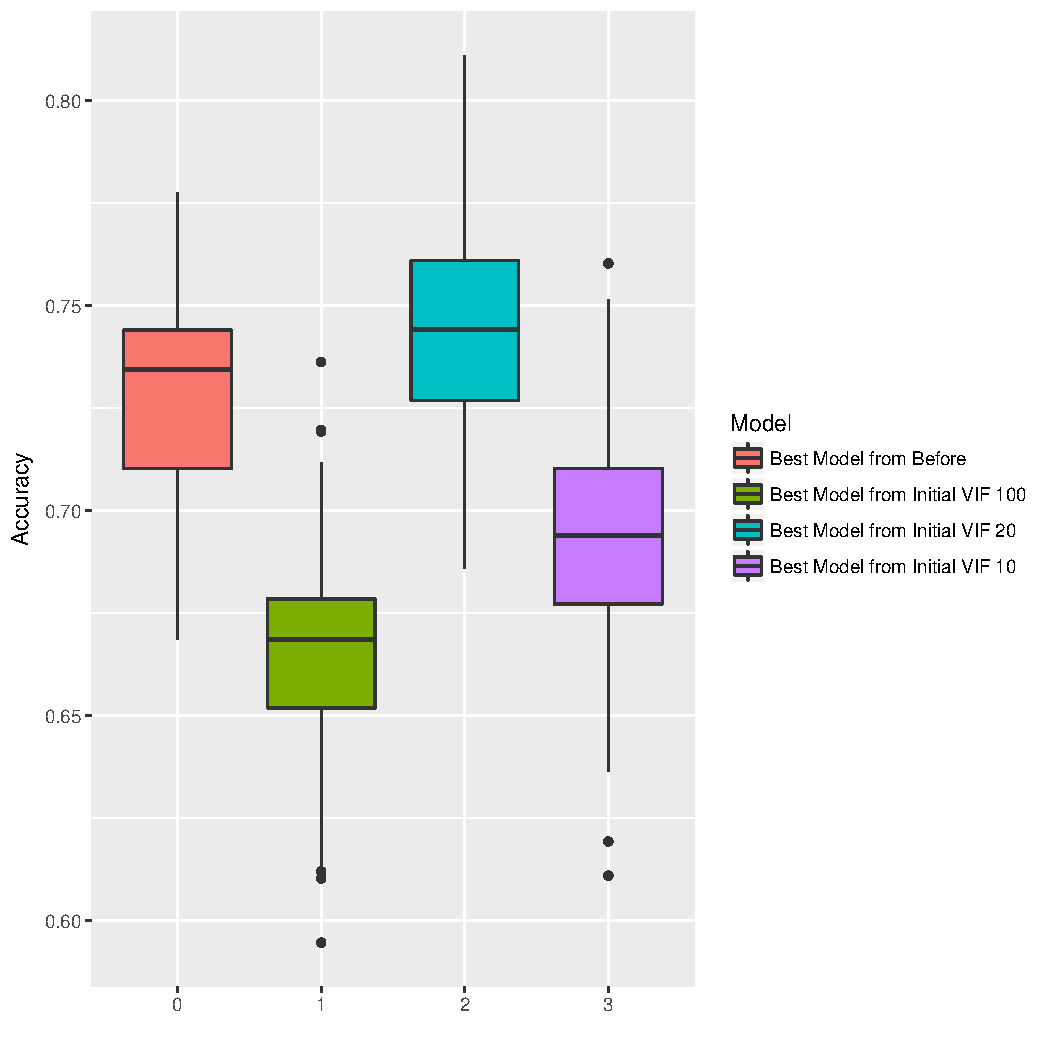
\includegraphics[width=\maxwidth]{figure/FigModelCrossVal3-1} \caption[Mean accuracy achieved during cross-validation]{Mean accuracy achieved during cross-validation. The minimal model still does as well as before removing the extra stains.}\label{fig:FigModelCrossVal3}
\end{figure}


\end{knitrout}

The one starting from maxVIF=20 seems to be much better than the others. It has 13 variables, the one from VIF10 has 12. What is the difference?
\begin{knitrout}
\definecolor{shadecolor}{rgb}{0.969, 0.969, 0.969}\color{fgcolor}\begin{kframe}
\begin{alltt}
\hlstd{both}\hlkwb{=}\hlkwd{names}\hlstd{(best10Model}\hlopt{$}\hlstd{coefficients)} \hlopt \hlkwd{names}\hlstd{(best20Model}\hlopt{$}\hlstd{coefficients)}
\hlkwd{names}\hlstd{(best10Model}\hlopt{$}\hlstd{coefficients)[both]}
\end{alltt}
\begin{verbatim}
##  [1] "(Intercept)"  "Vimentin"     "CD16"         "CD134"       
##  [5] "CD44s"        "`E-cadherin`" "p21"          "CD152"       
##  [9] "HistoneH3"    "DNA191"
\end{verbatim}
\end{kframe}
\end{knitrout}

So, they share 10 variables. Model20 in addition contains:

\begin{knitrout}
\definecolor{shadecolor}{rgb}{0.969, 0.969, 0.969}\color{fgcolor}\begin{kframe}
\begin{alltt}
\hlstd{only20} \hlkwb{=} \hlopt{!}\hlstd{(}\hlkwd{names}\hlstd{(best20Model}\hlopt{$}\hlstd{coefficients)} \hlopt \hlkwd{names}\hlstd{(best10Model}\hlopt{$}\hlstd{coefficients))}
\hlkwd{names}\hlstd{(best20Model}\hlopt{$}\hlstd{coefficients)[only20]}
\end{alltt}
\begin{verbatim}
## [1] "CD196" "CD19"  "CD25"  "pS6"
\end{verbatim}
\end{kframe}
\end{knitrout}

Whereas Model 10 contains:
\begin{knitrout}
\definecolor{shadecolor}{rgb}{0.969, 0.969, 0.969}\color{fgcolor}\begin{kframe}
\begin{alltt}
\hlkwd{names}\hlstd{(best10Model}\hlopt{$}\hlstd{coefficients)[}\hlopt{!}\hlstd{both]}
\end{alltt}
\begin{verbatim}
## [1] "CD14"      "`B7-H4`"   "CollagenI"
\end{verbatim}
\end{kframe}
\end{knitrout}

What do they look like?
\begin{knitrout}
\definecolor{shadecolor}{rgb}{0.969, 0.969, 0.969}\color{fgcolor}\begin{kframe}
\begin{alltt}
\hlstd{p} \hlkwb{=} \hlkwd{PlotCoefficients}\hlstd{(best20Model,}\hlkwc{yLim}\hlstd{=}\hlkwd{c}\hlstd{(}\hlopt{-}\hlnum{50}\hlstd{,}\hlnum{50}\hlstd{),}\hlkwc{yPos}\hlstd{=}\hlnum{22}\hlstd{,}\hlkwc{errBarWidth}\hlstd{=}\hlnum{.4}\hlstd{)}
\hlcom{# Annotate the markers}
\hlstd{yPos} \hlkwb{=} \hlnum{37}
\hlstd{tSize} \hlkwb{=} \hlnum{2.5}
\hlcom{# Positive}
\hlstd{p} \hlkwb{=} \hlstd{p} \hlopt{+} \hlkwd{annotate}\hlstd{(}\hlstr{"text"}\hlstd{,} \hlkwc{x} \hlstd{=} \hlstr{"CD196"}\hlstd{,} \hlkwc{y} \hlstd{= yPos,}
                       \hlkwc{label} \hlstd{=} \hlstr{"Immature Dendritic Cells/\textbackslash{}n Memory T-Cells"}\hlstd{,} \hlkwc{size} \hlstd{= tSize)}
\hlstd{p} \hlkwb{=} \hlstd{p} \hlopt{+} \hlkwd{annotate}\hlstd{(}\hlstr{"text"}\hlstd{,} \hlkwc{x} \hlstd{=} \hlstr{"CD19"}\hlstd{,} \hlkwc{y} \hlstd{= yPos,}
                       \hlkwc{label} \hlstd{=} \hlstr{"B-Cells"}\hlstd{,} \hlkwc{size} \hlstd{= tSize)}
\hlstd{p} \hlkwb{=} \hlstd{p} \hlopt{+} \hlkwd{annotate}\hlstd{(}\hlstr{"text"}\hlstd{,} \hlkwc{x} \hlstd{=} \hlstr{"`E-cadherin`"}\hlstd{,} \hlkwc{y} \hlstd{= yPos,}
                       \hlkwc{label} \hlstd{=} \hlstr{"Epithelial Phenotype"}\hlstd{,} \hlkwc{size} \hlstd{= tSize)}
\hlstd{p} \hlkwb{=} \hlstd{p} \hlopt{+} \hlkwd{annotate}\hlstd{(}\hlstr{"text"}\hlstd{,} \hlkwc{x} \hlstd{=} \hlstr{"HistoneH3"}\hlstd{,} \hlkwc{y} \hlstd{= yPos,}
                       \hlkwc{label} \hlstd{=} \hlstr{"Generic Cell Marker"}\hlstd{,} \hlkwc{size} \hlstd{= tSize)}
\hlstd{p} \hlkwb{=} \hlstd{p} \hlopt{+} \hlkwd{annotate}\hlstd{(}\hlstr{"text"}\hlstd{,} \hlkwc{x} \hlstd{=} \hlstr{"p21"}\hlstd{,} \hlkwc{y} \hlstd{= yPos,}
                       \hlkwc{label} \hlstd{=} \hlstr{"Cell Cycle Inhibitor"}\hlstd{,} \hlkwc{size} \hlstd{= tSize)}
\hlstd{p} \hlkwb{=} \hlstd{p} \hlopt{+} \hlkwd{annotate}\hlstd{(}\hlstr{"text"}\hlstd{,} \hlkwc{x} \hlstd{=} \hlstr{"DNA191"}\hlstd{,} \hlkwc{y} \hlstd{= yPos,}
                       \hlkwc{label} \hlstd{=} \hlstr{"NA"}\hlstd{,} \hlkwc{size} \hlstd{= tSize)}
\hlstd{p} \hlkwb{=} \hlstd{p} \hlopt{+} \hlkwd{annotate}\hlstd{(}\hlstr{"text"}\hlstd{,} \hlkwc{x} \hlstd{=} \hlstr{"DNA191"}\hlstd{,} \hlkwc{y} \hlstd{= yPos,}
                       \hlkwc{label} \hlstd{=} \hlstr{"NA"}\hlstd{,} \hlkwc{size} \hlstd{= tSize)}
\hlstd{p} \hlkwb{=} \hlstd{p} \hlopt{+} \hlkwd{annotate}\hlstd{(}\hlstr{"text"}\hlstd{,} \hlkwc{x} \hlstd{=} \hlstr{"CD44s"}\hlstd{,} \hlkwc{y} \hlstd{= yPos,}
                       \hlkwc{label} \hlstd{=} \hlstr{"Cell-Cell Interaction"}\hlstd{,} \hlkwc{size} \hlstd{= tSize)}
\hlstd{p} \hlkwb{=} \hlstd{p} \hlopt{+} \hlkwd{geom_rect}\hlstd{(}\hlkwd{aes}\hlstd{(}\hlkwc{xmin} \hlstd{=} \hlstr{"Vimentin"}\hlstd{,} \hlkwc{xmax} \hlstd{=} \hlnum{13.5}\hlstd{,} \hlkwc{ymin} \hlstd{=} \hlnum{25}\hlstd{,} \hlkwc{ymax} \hlstd{=} \hlnum{50}\hlstd{),}
               \hlkwc{fill} \hlstd{=} \hlstr{"transparent"}\hlstd{,} \hlkwc{color} \hlstd{=} \hlstr{"green4"}\hlstd{,} \hlkwc{size} \hlstd{=} \hlnum{1.5}\hlstd{)}

\hlcom{# Negative}
\hlstd{yPos} \hlkwb{=} \hlopt{-}\hlnum{37}
\hlstd{p} \hlkwb{=} \hlstd{p} \hlopt{+} \hlkwd{annotate}\hlstd{(}\hlstr{"text"}\hlstd{,} \hlkwc{x} \hlstd{=} \hlstr{"Vimentin"}\hlstd{,} \hlkwc{y} \hlstd{= yPos,}
                       \hlkwc{label} \hlstd{=} \hlstr{"Mesenchymal Phenotype"}\hlstd{,} \hlkwc{size} \hlstd{= tSize)}
\hlstd{p} \hlkwb{=} \hlstd{p} \hlopt{+} \hlkwd{annotate}\hlstd{(}\hlstr{"text"}\hlstd{,} \hlkwc{x} \hlstd{=} \hlstr{"pS6"}\hlstd{,} \hlkwc{y} \hlstd{= yPos,}
                       \hlkwc{label} \hlstd{=} \hlstr{"Increased Translation"}\hlstd{,} \hlkwc{size} \hlstd{= tSize)}
\hlstd{p} \hlkwb{=} \hlstd{p} \hlopt{+} \hlkwd{annotate}\hlstd{(}\hlstr{"text"}\hlstd{,} \hlkwc{x} \hlstd{=} \hlstr{"CD16"}\hlstd{,} \hlkwc{y} \hlstd{= yPos,}
                       \hlkwc{label} \hlstd{=} \hlstr{"Monocytes/\textbackslash{}n Macrophages/\textbackslash{}n NK Cells"}\hlstd{,} \hlkwc{size} \hlstd{= tSize)}
\hlstd{p} \hlkwb{=} \hlstd{p} \hlopt{+} \hlkwd{annotate}\hlstd{(}\hlstr{"text"}\hlstd{,} \hlkwc{x} \hlstd{=} \hlstr{"CD134"}\hlstd{,} \hlkwc{y} \hlstd{= yPos,}
                       \hlkwc{label} \hlstd{=} \hlstr{"T-Cell Activation\textbackslash{}n Survival"}\hlstd{,} \hlkwc{size} \hlstd{= tSize)}
\hlstd{p} \hlkwb{=} \hlstd{p} \hlopt{+} \hlkwd{annotate}\hlstd{(}\hlstr{"text"}\hlstd{,} \hlkwc{x} \hlstd{=} \hlstr{"CD152"}\hlstd{,} \hlkwc{y} \hlstd{= yPos,}
                       \hlkwc{label} \hlstd{=} \hlstr{"Checkpoint Inhibitor"}\hlstd{,} \hlkwc{size} \hlstd{= tSize)}
\hlstd{p} \hlkwb{=} \hlstd{p} \hlopt{+} \hlkwd{annotate}\hlstd{(}\hlstr{"text"}\hlstd{,} \hlkwc{x} \hlstd{=} \hlstr{"CD25"}\hlstd{,} \hlkwc{y} \hlstd{= yPos,}
                       \hlkwc{label} \hlstd{=} \hlstr{"Activated T- and B-Cells"}\hlstd{,} \hlkwc{size} \hlstd{= tSize)}
\hlstd{p} \hlkwb{=} \hlstd{p} \hlopt{+} \hlkwd{geom_rect}\hlstd{(}\hlkwd{aes}\hlstd{(}\hlkwc{xmin} \hlstd{=} \hlnum{0}\hlstd{,} \hlkwc{xmax} \hlstd{=} \hlstr{"CD44s"}\hlstd{,} \hlkwc{ymin} \hlstd{=} \hlopt{-}\hlnum{25}\hlstd{,} \hlkwc{ymax} \hlstd{=} \hlopt{-}\hlnum{50}\hlstd{),}
               \hlkwc{fill} \hlstd{=} \hlstr{"transparent"}\hlstd{,} \hlkwc{color} \hlstd{=} \hlstr{"red"}\hlstd{,} \hlkwc{size} \hlstd{=} \hlnum{1.5}\hlstd{)}

\hlstd{p}
\end{alltt}
\end{kframe}\begin{figure}[h]
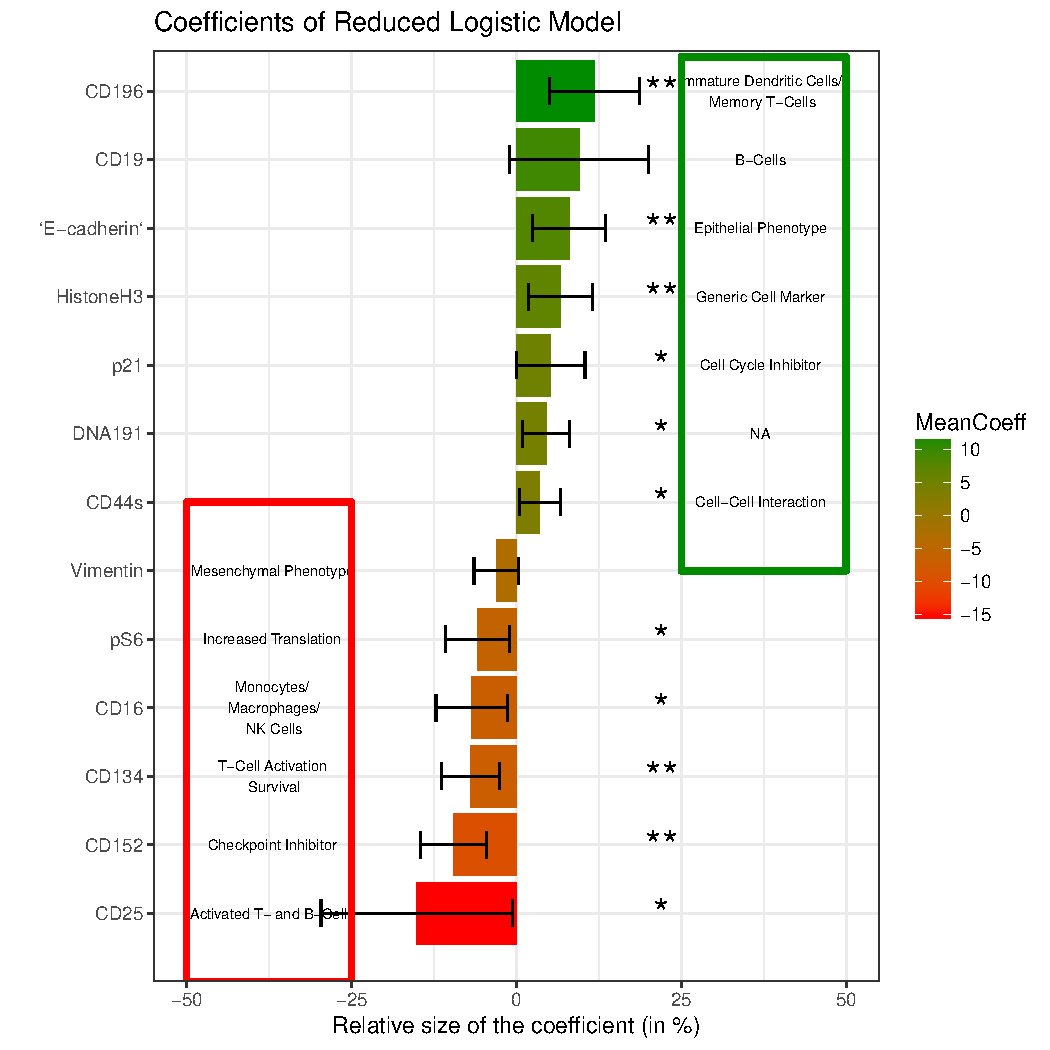
\includegraphics[width=\maxwidth]{figure/Fig_Model20-1} \caption[Importance of the different stains according to the logistic model with maxVIF 20]{Importance of the different stains according to the logistic model with maxVIF 20. Asterisk indicates level of statistical support for non-zero contribution from this stain (T-test: *p$<$0.05,**p$<$0.01).}\label{fig:Fig_Model20}
\end{figure}


\end{knitrout}

So this model is almost the one I got previously, just with fewer variables. Interestingly it seems to be even more robust in the cross-validation.

Let's look at model10:
\begin{knitrout}
\definecolor{shadecolor}{rgb}{0.969, 0.969, 0.969}\color{fgcolor}\begin{kframe}
\begin{alltt}
\hlkwd{PlotCoefficients}\hlstd{(best10Model,}\hlkwc{yLim}\hlstd{=}\hlkwd{c}\hlstd{(}\hlopt{-}\hlnum{30}\hlstd{,}\hlnum{30}\hlstd{),}\hlkwc{yPos}\hlstd{=}\hlnum{22}\hlstd{,}\hlkwc{errBarWidth}\hlstd{=}\hlnum{.4}\hlstd{)}
\end{alltt}
\end{kframe}\begin{figure}[h]
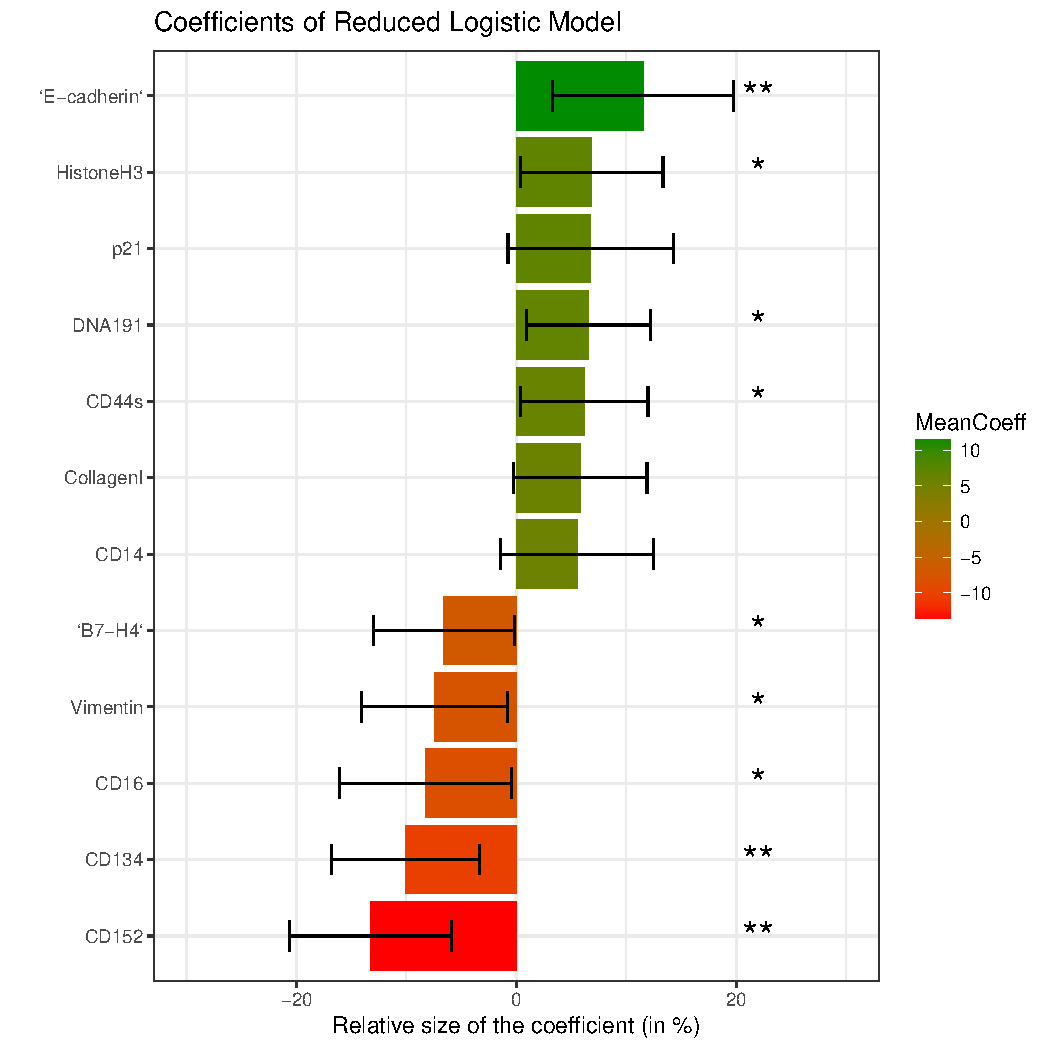
\includegraphics[width=\maxwidth]{figure/Fig_Model10-1} \caption[Importance of the different stains according to the logistic model with maxVIF 10]{Importance of the different stains according to the logistic model with maxVIF 10. Asterisk indicates level of statistical support for non-zero contribution from this stain (T-test: *p$<$0.05,**p$<$0.01).}\label{fig:Fig_Model10}
\end{figure}


\end{knitrout}

Yeah, that doesn't look as nice. Strange it wants CD14 and CollagenI when they're not significant...

As of now the one I prefer most is probably model20, which has the best AIC and still okish VIFs. The AIC of the model from the previous section was 132.4854583, model20 has an AIC of 135.5028521. So the AIC is slightly worse, but interestingly it's performance in cross-validation is slightly better. It's VIFs are also much better (max now is around 20, before it was 40. It's strange though that we're now picking up Histones...

Just for completeness, here are its summary and vifs:
\begin{knitrout}
\definecolor{shadecolor}{rgb}{0.969, 0.969, 0.969}\color{fgcolor}\begin{kframe}
\begin{alltt}
\hlkwd{summary}\hlstd{(best20Model)}
\end{alltt}
\begin{verbatim}
## 
## Call:
## glm(formula = paste0(best20[, 5]), family = binomial(link = "logit"), 
##     data = meanStainWide_Tranformed)
## 
## Deviance Residuals: 
##     Min       1Q   Median       3Q      Max  
## -2.4763  -0.6551   0.3236   0.7700   1.7136  
## 
## Coefficients:
##              Estimate Std. Error z value Pr(>|z|)    
## (Intercept)    0.6869     0.2732   2.515 0.011914 *  
## CD196          2.3959     0.6937   3.454 0.000553 ***
## CD19           1.9217     1.0768   1.785 0.074327 .  
## Vimentin      -0.6173     0.3453  -1.788 0.073831 .  
## CD16          -1.3708     0.5502  -2.491 0.012728 *  
## CD25          -3.0547     1.4827  -2.060 0.039374 *  
## CD134         -1.4028     0.4497  -3.119 0.001812 ** 
## CD44s          0.7172     0.3163   2.267 0.023367 *  
## `E-cadherin`   1.6189     0.5664   2.858 0.004263 ** 
## p21            1.0554     0.5275   2.001 0.045405 *  
## CD152         -1.9252     0.5151  -3.737 0.000186 ***
## pS6           -1.1860     0.4982  -2.381 0.017276 *  
## HistoneH3      1.3485     0.4960   2.719 0.006551 ** 
## DNA191         0.9156     0.3626   2.525 0.011572 *  
## ---
## Signif. codes:  0 '***' 0.001 '**' 0.01 '*' 0.05 '.' 0.1 ' ' 1
## 
## (Dispersion parameter for binomial family taken to be 1)
## 
##     Null deviance: 161.67  on 120  degrees of freedom
## Residual deviance: 107.50  on 107  degrees of freedom
## AIC: 135.5
## 
## Number of Fisher Scoring iterations: 6
\end{verbatim}
\begin{alltt}
\hlstd{vifVec} \hlkwb{=} \hlkwd{vif}\hlstd{(best20Model)}
\hlstd{vifVec[}\hlkwd{order}\hlstd{(vifVec,}\hlkwc{decreasing}\hlstd{=T)]}
\end{alltt}
\begin{verbatim}
##         CD25         CD19        CD152 `E-cadherin`        CD196 
##    21.542411    19.233730     4.287444     4.119309     4.010219 
##          p21    HistoneH3         CD16          pS6        CD134 
##     3.899845     3.642846     3.495984     3.477955     2.895262 
##       DNA191     Vimentin        CD44s 
##     2.446263     1.709218     1.623995
\end{verbatim}
\end{kframe}
\end{knitrout}

Actually, CD25 and CD19 seem to be the two variables with problematic VIFs. Maybe that's why their standard errors are inflated? What happens if I remove them? The current aic is 135.5028521

\begin{knitrout}
\definecolor{shadecolor}{rgb}{0.969, 0.969, 0.969}\color{fgcolor}\begin{kframe}
\begin{alltt}
\hlstd{best20Model_NoCd25} \hlkwb{=} \hlkwd{update}\hlstd{(best20Model,.}\hlopt{~}\hlstd{.}\hlopt{-}\hlstd{CD25)}
\hlkwd{summary}\hlstd{(best20Model_NoCd25)}
\end{alltt}
\begin{verbatim}
## 
## Call:
## glm(formula = PtSnty ~ CD196 + CD19 + Vimentin + CD16 + CD134 + 
##     CD44s + `E-cadherin` + p21 + CD152 + pS6 + HistoneH3 + DNA191, 
##     family = binomial(link = "logit"), data = meanStainWide_Tranformed)
## 
## Deviance Residuals: 
##     Min       1Q   Median       3Q      Max  
## -2.6323  -0.8634   0.4275   0.8766   1.5048  
## 
## Coefficients:
##              Estimate Std. Error z value Pr(>|z|)    
## (Intercept)    0.5796     0.2298   2.523 0.011644 *  
## CD196          0.5968     0.3869   1.543 0.122943    
## CD19           0.1235     0.3058   0.404 0.686281    
## Vimentin      -0.4544     0.3000  -1.515 0.129832    
## CD16          -1.2205     0.4910  -2.486 0.012925 *  
## CD134         -0.8689     0.3481  -2.496 0.012563 *  
## CD44s          0.6941     0.3138   2.212 0.026972 *  
## `E-cadherin`   1.3152     0.4747   2.770 0.005598 ** 
## p21            0.4352     0.4377   0.994 0.319988    
## CD152         -1.4589     0.4221  -3.456 0.000548 ***
## pS6           -0.1960     0.3547  -0.553 0.580479    
## HistoneH3      0.8023     0.3785   2.120 0.034046 *  
## DNA191         0.6942     0.3233   2.147 0.031781 *  
## ---
## Signif. codes:  0 '***' 0.001 '**' 0.01 '*' 0.05 '.' 0.1 ' ' 1
## 
## (Dispersion parameter for binomial family taken to be 1)
## 
##     Null deviance: 161.67  on 120  degrees of freedom
## Residual deviance: 124.76  on 108  degrees of freedom
## AIC: 150.76
## 
## Number of Fisher Scoring iterations: 5
\end{verbatim}
\begin{alltt}
\hlstd{vifVec} \hlkwb{=} \hlkwd{vif}\hlstd{(best20Model_NoCd25)}
\hlstd{vifVec[}\hlkwd{order}\hlstd{(vifVec,}\hlkwc{decreasing}\hlstd{=T)]}
\end{alltt}
\begin{verbatim}
##        CD152 `E-cadherin`          p21         CD16    HistoneH3 
##     3.701210     3.680306     3.417115     3.410232     2.875400 
##       DNA191        CD134          pS6         CD19        CD196 
##     2.268048     2.126973     1.926199     1.892555     1.642036 
##        CD44s     Vimentin 
##     1.531749     1.473587
\end{verbatim}
\end{kframe}
\end{knitrout}

The model is much worse now, but the VIFs are fine... What if I remove CD19 instead?

\begin{knitrout}
\definecolor{shadecolor}{rgb}{0.969, 0.969, 0.969}\color{fgcolor}\begin{kframe}
\begin{alltt}
\hlstd{best20Model_NoCd19} \hlkwb{=} \hlkwd{update}\hlstd{(best20Model,.}\hlopt{~}\hlstd{.}\hlopt{-}\hlstd{CD19)}
\hlkwd{summary}\hlstd{(best20Model_NoCd19)}
\end{alltt}
\begin{verbatim}
## 
## Call:
## glm(formula = PtSnty ~ CD196 + Vimentin + CD16 + CD25 + CD134 + 
##     CD44s + `E-cadherin` + p21 + CD152 + pS6 + HistoneH3 + DNA191, 
##     family = binomial(link = "logit"), data = meanStainWide_Tranformed)
## 
## Deviance Residuals: 
##     Min       1Q   Median       3Q      Max  
## -2.6014  -0.8309   0.3938   0.8164   1.8306  
## 
## Coefficients:
##              Estimate Std. Error z value Pr(>|z|)    
## (Intercept)    0.6160     0.2340   2.632 0.008488 ** 
## CD196          1.2877     0.4765   2.702 0.006884 ** 
## Vimentin      -0.5399     0.3151  -1.713 0.086667 .  
## CD16          -0.8398     0.4169  -2.014 0.043965 *  
## CD25          -0.9455     0.4294  -2.202 0.027682 *  
## CD134         -0.8970     0.3522  -2.547 0.010874 *  
## CD44s          0.7196     0.3100   2.321 0.020270 *  
## `E-cadherin`   1.1315     0.4537   2.494 0.012626 *  
## p21            0.6626     0.4492   1.475 0.140233    
## CD152         -1.4919     0.4260  -3.502 0.000461 ***
## pS6           -0.5130     0.3812  -1.346 0.178413    
## HistoneH3      0.8906     0.3997   2.228 0.025893 *  
## DNA191         0.7998     0.3377   2.369 0.017859 *  
## ---
## Signif. codes:  0 '***' 0.001 '**' 0.01 '*' 0.05 '.' 0.1 ' ' 1
## 
## (Dispersion parameter for binomial family taken to be 1)
## 
##     Null deviance: 161.67  on 120  degrees of freedom
## Residual deviance: 119.59  on 108  degrees of freedom
## AIC: 145.59
## 
## Number of Fisher Scoring iterations: 5
\end{verbatim}
\end{kframe}
\end{knitrout}

Not really a huge improvement either...
Yeah, let's leave it here for now. This seems like a decent model

\section{Dependence of Platinum Response on Cancer Grade}
The results from the logisitic model are very interesting, because they suggest that it is less something about the cancer that makes the difference, but more the environment. However, it is clear that the environment does change over time and what might be good early in cancer development might be bad later on. It is very plausible that the precise influence of, for example, the immune system is very dependent on the stage of the tumour. This could also explain the large error bars for some of the coefficients. Perhaps, stains like CD25 are very important for a sub-part of the patients but not others.

In order to see how our results depend on the tumour class, let's incorporate them into the model.
To do so I first have to associate each core with its grade.
\begin{knitrout}
\definecolor{shadecolor}{rgb}{0.969, 0.969, 0.969}\color{fgcolor}\begin{kframe}
\begin{alltt}
\hlstd{patientDB} \hlkwb{=} \hlkwd{read.csv}\hlstd{(}\hlstr{"fluidigm_patient_response.csv"}\hlstd{)}

\hlstd{meanStain_Staged} \hlkwb{=} \hlkwd{data.frame}\hlstd{(}\hlkwc{CoreId}\hlstd{=meanStain_Wide}\hlopt{$}\hlstd{CoreId,meanStainWide_Tranformed,}\hlkwc{Stage}\hlstd{=}\hlkwd{rep}\hlstd{(}\hlnum{0}\hlstd{,}\hlkwd{nrow}\hlstd{(meanStain_Wide)))}

\hlkwa{for} \hlstd{(coreId} \hlkwa{in} \hlstd{meanStain_Staged}\hlopt{$}\hlstd{CoreId)\{}
  \hlstd{patientId} \hlkwb{=} \hlkwd{which}\hlstd{(patientDB}\hlopt{$}\hlstd{core.1}\hlopt{==}\hlstd{coreId)}
  \hlkwa{if}\hlstd{(}\hlkwd{length}\hlstd{(patientId)}\hlopt{==}\hlnum{0}\hlstd{) patientId} \hlkwb{=} \hlkwd{which}\hlstd{(patientDB}\hlopt{$}\hlstd{core.2}\hlopt{==}\hlstd{coreId)}

  \hlcom{# Stage the patient}
  \hlstd{stage} \hlkwb{=} \hlstd{patientDB}\hlopt{$}\hlstd{stage[patientId]}
  \hlstd{meanStain_Staged}\hlopt{$}\hlstd{Stage[meanStain_Staged}\hlopt{$}\hlstd{CoreId}\hlopt{==}\hlstd{coreId]} \hlkwb{=} \hlstd{stage}
  \hlkwd{print}\hlstd{(}\hlkwd{paste}\hlstd{(patientId,stage))}
\hlstd{\}}
\end{alltt}
\begin{verbatim}
## [1] "52 4"
## [1] "43 3C"
## [1] "2 3C"
## [1] "35 3C"
## [1] "64 3C"
## [1] "6 3C"
## [1] "38 2C"
## [1] "60 3A"
## [1] "14 3C"
## [1] "67 3A"
## [1] "51 3C"
## [1] "45 3C"
## [1] "29 3C"
## [1] "38 2C"
## [1] "31 3C"
## [1] "61 3C"
## [1] "9 4"
## [1] "52 4"
## [1] "30 3C"
## [1] "11 3C"
## [1] "24 3C"
## [1] "13 3B"
## [1] "46 3C"
## [1] "28 3A"
## [1] "19 3C"
## [1] "12 4"
## [1] "62 3C"
## [1] "58 3C"
## [1] "41 3C"
## [1] "55 3C"
## [1] "65 3B"
## [1] "31 3C"
## [1] "53 4"
## [1] "27 3C"
## [1] "21 3C"
## [1] "40 2C"
## [1] "47 3C"
## [1] "54 3C"
## [1] "37 1C"
## [1] "7 3C"
## [1] "49 3C"
## [1] "32 4"
## [1] "8 3B"
## [1] "15 4"
## [1] "66 3C"
## [1] "1 3C"
## [1] "39 1C"
## [1] "2 3C"
## [1] "57 3C"
## [1] "36 4"
## [1] "48 3A"
## [1] "3 3A"
## [1] "49 3C"
## [1] "61 3C"
## [1] "17 3C"
## [1] "23 4"
## [1] "50 4"
## [1] "60 3A"
## [1] "56 3C"
## [1] "59 3C"
## [1] "41 3C"
## [1] "34 3C"
## [1] "30 3C"
## [1] "33 3C"
## [1] "6 3C"
## [1] "64 3C"
## [1] "22 3C"
## [1] "25 3C"
## [1] "5 4"
## [1] "20 3C"
## [1] "24 3C"
## [1] "16 3C"
## [1] "10 4"
## [1] "26 2C"
## [1] "4 3C"
## [1] "16 3C"
## [1] "51 3C"
## [1] "45 3C"
## [1] "63 4"
## [1] "1 3C"
## [1] "23 4"
## [1] "32 4"
## [1] "36 4"
## [1] "28 3A"
## [1] "66 3C"
## [1] "4 3C"
## [1] "11 3C"
## [1] "21 3C"
## [1] "29 3C"
## [1] "53 4"
## [1] "67 3A"
## [1] "50 4"
## [1] "10 4"
## [1] "47 3C"
## [1] "22 3C"
## [1] "59 3C"
## [1] "55 3C"
## [1] "27 3C"
## [1] "42 2C"
## [1] "44 2B"
## [1] "57 3C"
## [1] "39 1C"
## [1] "62 3C"
## [1] "8 3B"
## [1] "7 3C"
## [1] "68 3C"
## [1] "12 4"
## [1] "37 1C"
## [1] "58 3C"
## [1] "15 4"
## [1] "13 3B"
## [1] "26 2C"
## [1] "19 3C"
## [1] "25 3C"
## [1] "54 3C"
## [1] "3 3A"
## [1] "5 4"
## [1] "34 3C"
## [1] "56 3C"
## [1] "20 3C"
## [1] "68 3C"
\end{verbatim}
\begin{alltt}
\hlstd{meanStain_Staged}\hlopt{$}\hlstd{Stage} \hlkwb{=} \hlkwd{as.factor}\hlstd{(meanStain_Staged}\hlopt{$}\hlstd{Stage)}
\hlkwd{levels}\hlstd{(meanStain_Staged}\hlopt{$}\hlstd{Stage)} \hlkwb{=} \hlkwd{levels}\hlstd{(patientDB}\hlopt{$}\hlstd{stage)}
\hlkwd{summary}\hlstd{(meanStain_Staged}\hlopt{$}\hlstd{Stage)}
\end{alltt}
\begin{verbatim}
## 1C 2B 2C 3A 3B 3C  4 
##  4  1  6  9  5 74 22
\end{verbatim}
\end{kframe}
\end{knitrout}

This does suggest a heavy skew towards patients with stage 3C and 4 cancer. This might make the analysis difficult, but maybe if we group accordingly we can pull something out. The cancer grading works as follows:
\begin{itemize}
\item Stage I: Local disease confined to the ovaries
\item Stage II: Cancer has spread to other pelvic structures (e.g. uterus, fallopian tubes, bladder, the sigmoid colon, or the rectum). But not lymph nodes or distant sides.
\item Stage III: Cancer has spread to the abdomen and/or the draining nodal beds.
\item Stage IV: Metastatic Lesions outside the abdomen (e.g. liver or lung).
\end{itemize}

For a detailed breakdown see https://www.cancer.org/cancer/ovarian-cancer/detection-diagnosis-staging/staging.html.

Let's make 4 groups for now and then take it from there.

\begin{knitrout}
\definecolor{shadecolor}{rgb}{0.969, 0.969, 0.969}\color{fgcolor}\begin{kframe}
\begin{alltt}
\hlstd{meanStain_Staged}\hlopt{$}\hlstd{StageCoarse[meanStain_Staged}\hlopt{$}\hlstd{Stage}\hlopt{==}\hlstr{"1C"}\hlstd{]} \hlkwb{=} \hlnum{1}
\hlstd{meanStain_Staged}\hlopt{$}\hlstd{StageCoarse[meanStain_Staged}\hlopt{$}\hlstd{Stage}\hlopt{==}\hlstr{"2B"}\hlstd{]} \hlkwb{=} \hlnum{2}
\hlstd{meanStain_Staged}\hlopt{$}\hlstd{StageCoarse[meanStain_Staged}\hlopt{$}\hlstd{Stage}\hlopt{==}\hlstr{"2C"}\hlstd{]} \hlkwb{=} \hlnum{2}
\hlstd{meanStain_Staged}\hlopt{$}\hlstd{StageCoarse[meanStain_Staged}\hlopt{$}\hlstd{Stage}\hlopt{==}\hlstr{"3A"}\hlstd{]} \hlkwb{=} \hlnum{3}
\hlstd{meanStain_Staged}\hlopt{$}\hlstd{StageCoarse[meanStain_Staged}\hlopt{$}\hlstd{Stage}\hlopt{==}\hlstr{"3B"}\hlstd{]} \hlkwb{=} \hlnum{3}
\hlstd{meanStain_Staged}\hlopt{$}\hlstd{StageCoarse[meanStain_Staged}\hlopt{$}\hlstd{Stage}\hlopt{==}\hlstr{"3C"}\hlstd{]} \hlkwb{=} \hlnum{3}
\hlstd{meanStain_Staged}\hlopt{$}\hlstd{StageCoarse[meanStain_Staged}\hlopt{$}\hlstd{Stage}\hlopt{==}\hlstr{"4"}\hlstd{]} \hlkwb{=} \hlnum{4}
\end{alltt}
\end{kframe}
\end{knitrout}

Start the modelling process. For now let's model grade as a continous variable.
\begin{knitrout}
\definecolor{shadecolor}{rgb}{0.969, 0.969, 0.969}\color{fgcolor}\begin{kframe}
\begin{alltt}
\hlstd{meanStain_Staged}\hlopt{$}\hlstd{StageCoarse} \hlkwb{=} \hlkwd{as.numeric}\hlstd{(meanStain_Staged}\hlopt{$}\hlstd{StageCoarse)}
\hlstd{omit} \hlkwb{=} \hlkwd{c}\hlstd{(}\hlkwd{which}\hlstd{(}\hlkwd{names}\hlstd{(meanStain_Staged)}\hlopt{==}\hlstr{"CoreId"}\hlstd{),}\hlkwd{which}\hlstd{(}\hlkwd{names}\hlstd{(meanStain_Staged)}\hlopt{==}\hlstr{"Stage"}\hlstd{))}
\hlstd{initModel} \hlkwb{=} \hlkwd{glm}\hlstd{(PtSnty} \hlopt{~}\hlstd{.,}\hlkwc{family}\hlstd{=}\hlkwd{binomial}\hlstd{(}\hlkwc{link}\hlstd{=}\hlstr{'logit'}\hlstd{),}
                    \hlkwc{data}\hlstd{=meanStain_Staged[,}\hlopt{-}\hlstd{omit])}
\hlstd{stagedModelArr} \hlkwb{=} \hlkwd{AICVIFCoElimination}\hlstd{(}\hlkwd{DecorrelateVariables}\hlstd{(initModel,}\hlnum{100}\hlstd{,}\hlkwc{verbose}\hlstd{=F)}
                                              \hlstd{,}\hlkwc{verbose}\hlstd{=F)}
\hlstd{stagedModel} \hlkwb{=} \hlkwd{glm}\hlstd{(}\hlkwd{paste0}\hlstd{(stagedModelArr[}\hlnum{4}\hlstd{,}\hlnum{5}\hlstd{]),}\hlkwc{family}\hlstd{=}\hlkwd{binomial}\hlstd{(}\hlkwc{link}\hlstd{=}\hlstr{'logit'}\hlstd{),}
                    \hlkwc{data}\hlstd{=meanStain_Staged[,}\hlopt{-}\hlstd{omit])}
\hlkwd{summary}\hlstd{(stagedModel)}
\end{alltt}
\begin{verbatim}
## 
## Call:
## glm(formula = paste0(stagedModelArr[4, 5]), family = binomial(link = "logit"), 
##     data = meanStain_Staged[, -omit])
## 
## Deviance Residuals: 
##     Min       1Q   Median       3Q      Max  
## -2.1026  -0.9572   0.5239   0.8957   1.5171  
## 
## Coefficients:
##             Estimate Std. Error z value Pr(>|z|)   
## (Intercept)   3.4311     1.2694   2.703  0.00687 **
## CD196         0.4016     0.2675   1.501  0.13332   
## Vimentin     -0.7278     0.3011  -2.417  0.01564 * 
## CD16         -0.7259     0.3578  -2.029  0.04244 * 
## CD134        -0.5320     0.2838  -1.874  0.06088 . 
## CD44s         0.7357     0.3073   2.394  0.01664 * 
## CD152        -0.9555     0.3316  -2.881  0.00396 **
## HistoneH3     1.0822     0.3549   3.049  0.00230 **
## DNA191        0.8239     0.3152   2.614  0.00896 **
## StageCoarse  -0.9408     0.4010  -2.346  0.01897 * 
## ---
## Signif. codes:  0 '***' 0.001 '**' 0.01 '*' 0.05 '.' 0.1 ' ' 1
## 
## (Dispersion parameter for binomial family taken to be 1)
## 
##     Null deviance: 161.67  on 120  degrees of freedom
## Residual deviance: 132.14  on 111  degrees of freedom
## AIC: 152.14
## 
## Number of Fisher Scoring iterations: 4
\end{verbatim}
\begin{alltt}
\hlkwd{vif}\hlstd{(stagedModel)}
\end{alltt}
\begin{verbatim}
##       CD196    Vimentin        CD16       CD134       CD44s       CD152 
##    1.410074    1.748973    2.257047    1.637027    1.602306    2.571201 
##   HistoneH3      DNA191 StageCoarse 
##    2.691540    2.224208    1.147944
\end{verbatim}
\end{kframe}
\end{knitrout}

Try interactions
\begin{knitrout}
\definecolor{shadecolor}{rgb}{0.969, 0.969, 0.969}\color{fgcolor}\begin{kframe}
\begin{alltt}
\hlstd{stagedModel} \hlkwb{=} \hlkwd{update}\hlstd{(stagedModel,.}\hlopt{~}\hlstd{.}\hlopt{+}\hlstd{StageCoarse}\hlopt{:}\hlstd{CD196}\hlopt{+}\hlstd{StageCoarse}\hlopt{:}\hlstd{Vimentin}\hlopt{+}
                       \hlstd{StageCoarse}\hlopt{:}\hlstd{CD16}\hlopt{+}\hlstd{StageCoarse}\hlopt{:}\hlstd{CD134}\hlopt{+}\hlstd{StageCoarse}\hlopt{:}\hlstd{CD44s}\hlopt{+}
                       \hlstd{StageCoarse}\hlopt{:}\hlstd{CD152}\hlopt{+}\hlstd{StageCoarse}\hlopt{:}\hlstd{HistoneH3}\hlopt{+}\hlstd{StageCoarse}\hlopt{:}\hlstd{DNA191)}
\hlstd{stagedModel}\hlkwb{=}\hlkwd{step}\hlstd{(stagedModel)}
\end{alltt}
\begin{verbatim}
## Start:  AIC=149.85
## PtSnty ~ CD196 + Vimentin + CD16 + CD134 + CD44s + CD152 + HistoneH3 + 
##     DNA191 + StageCoarse + CD196:StageCoarse + Vimentin:StageCoarse + 
##     CD16:StageCoarse + CD134:StageCoarse + CD44s:StageCoarse + 
##     CD152:StageCoarse + HistoneH3:StageCoarse + DNA191:StageCoarse
## 
##                         Df Deviance    AIC
## - CD44s:StageCoarse      1   113.86 147.86
## - CD134:StageCoarse      1   113.88 147.88
## - CD16:StageCoarse       1   113.93 147.93
## - CD152:StageCoarse      1   114.58 148.58
## - DNA191:StageCoarse     1   115.54 149.54
## <none>                       113.85 149.85
## - HistoneH3:StageCoarse  1   115.86 149.86
## - CD196:StageCoarse      1   122.11 156.11
## - Vimentin:StageCoarse   1   128.60 162.60
## 
## Step:  AIC=147.86
## PtSnty ~ CD196 + Vimentin + CD16 + CD134 + CD44s + CD152 + HistoneH3 + 
##     DNA191 + StageCoarse + CD196:StageCoarse + Vimentin:StageCoarse + 
##     CD16:StageCoarse + CD134:StageCoarse + CD152:StageCoarse + 
##     HistoneH3:StageCoarse + DNA191:StageCoarse
## 
##                         Df Deviance    AIC
## - CD134:StageCoarse      1   113.88 145.88
## - CD16:StageCoarse       1   113.96 145.96
## - CD152:StageCoarse      1   114.59 146.59
## - DNA191:StageCoarse     1   115.54 147.54
## <none>                       113.86 147.86
## - HistoneH3:StageCoarse  1   116.09 148.09
## - CD196:StageCoarse      1   122.29 154.29
## - CD44s                  1   122.60 154.60
## - Vimentin:StageCoarse   1   128.91 160.91
## 
## Step:  AIC=145.88
## PtSnty ~ CD196 + Vimentin + CD16 + CD134 + CD44s + CD152 + HistoneH3 + 
##     DNA191 + StageCoarse + CD196:StageCoarse + Vimentin:StageCoarse + 
##     CD16:StageCoarse + CD152:StageCoarse + HistoneH3:StageCoarse + 
##     DNA191:StageCoarse
## 
##                         Df Deviance    AIC
## - CD16:StageCoarse       1   113.98 143.98
## - CD152:StageCoarse      1   114.59 144.59
## - DNA191:StageCoarse     1   115.54 145.54
## <none>                       113.88 145.88
## - HistoneH3:StageCoarse  1   116.36 146.35
## - CD134                  1   119.00 149.00
## - CD196:StageCoarse      1   122.31 152.31
## - CD44s                  1   122.60 152.60
## - Vimentin:StageCoarse   1   128.91 158.91
## 
## Step:  AIC=143.98
## PtSnty ~ CD196 + Vimentin + CD16 + CD134 + CD44s + CD152 + HistoneH3 + 
##     DNA191 + StageCoarse + CD196:StageCoarse + Vimentin:StageCoarse + 
##     CD152:StageCoarse + HistoneH3:StageCoarse + DNA191:StageCoarse
## 
##                         Df Deviance    AIC
## - CD152:StageCoarse      1   114.70 142.70
## - DNA191:StageCoarse     1   115.79 143.79
## <none>                       113.98 143.98
## - HistoneH3:StageCoarse  1   117.21 145.21
## - CD16                   1   117.77 145.77
## - CD134                  1   119.11 147.11
## - CD196:StageCoarse      1   122.39 150.40
## - CD44s                  1   122.74 150.74
## - Vimentin:StageCoarse   1   129.34 157.34
## 
## Step:  AIC=142.7
## PtSnty ~ CD196 + Vimentin + CD16 + CD134 + CD44s + CD152 + HistoneH3 + 
##     DNA191 + StageCoarse + CD196:StageCoarse + Vimentin:StageCoarse + 
##     HistoneH3:StageCoarse + DNA191:StageCoarse
## 
##                         Df Deviance    AIC
## - DNA191:StageCoarse     1   115.89 141.89
## <none>                       114.70 142.70
## - HistoneH3:StageCoarse  1   117.23 143.23
## - CD16                   1   118.70 144.70
## - CD134                  1   119.55 145.55
## - CD196:StageCoarse      1   122.70 148.71
## - CD44s                  1   124.24 150.24
## - CD152                  1   124.24 150.24
## - Vimentin:StageCoarse   1   129.35 155.35
## 
## Step:  AIC=141.89
## PtSnty ~ CD196 + Vimentin + CD16 + CD134 + CD44s + CD152 + HistoneH3 + 
##     DNA191 + StageCoarse + CD196:StageCoarse + Vimentin:StageCoarse + 
##     HistoneH3:StageCoarse
## 
##                         Df Deviance    AIC
## <none>                       115.89 141.89
## - CD16                   1   119.72 143.72
## - CD134                  1   120.73 144.73
## - HistoneH3:StageCoarse  1   121.53 145.53
## - DNA191                 1   122.77 146.77
## - CD196:StageCoarse      1   124.21 148.21
## - CD44s                  1   125.26 149.26
## - CD152                  1   125.65 149.65
## - Vimentin:StageCoarse   1   130.26 154.26
\end{verbatim}
\begin{alltt}
\hlkwd{summary}\hlstd{(stagedModel)}
\end{alltt}
\begin{verbatim}
## 
## Call:
## glm(formula = PtSnty ~ CD196 + Vimentin + CD16 + CD134 + CD44s + 
##     CD152 + HistoneH3 + DNA191 + StageCoarse + CD196:StageCoarse + 
##     Vimentin:StageCoarse + HistoneH3:StageCoarse, family = binomial(link = "logit"), 
##     data = meanStain_Staged[, -omit])
## 
## Deviance Residuals: 
##     Min       1Q   Median       3Q      Max  
## -2.1184  -0.7847   0.3648   0.8307   2.0529  
## 
## Coefficients:
##                       Estimate Std. Error z value Pr(>|z|)   
## (Intercept)             6.0661     2.5064   2.420  0.01551 * 
## CD196                  -9.4343     4.5025  -2.095  0.03614 * 
## Vimentin               14.2187     6.5399   2.174  0.02969 * 
## CD16                   -0.6791     0.3903  -1.740  0.08182 . 
## CD134                  -0.6760     0.3468  -1.949  0.05125 . 
## CD44s                   0.8843     0.3402   2.600  0.00933 **
## CD152                  -1.0568     0.3614  -2.924  0.00346 **
## HistoneH3              -3.6442     2.2170  -1.644  0.10023   
## DNA191                  0.8763     0.3509   2.497  0.01251 * 
## StageCoarse            -1.8803     0.8241  -2.282  0.02251 * 
## CD196:StageCoarse       3.2846     1.4937   2.199  0.02788 * 
## Vimentin:StageCoarse   -5.0478     2.1751  -2.321  0.02030 * 
## HistoneH3:StageCoarse   1.6113     0.7384   2.182  0.02910 * 
## ---
## Signif. codes:  0 '***' 0.001 '**' 0.01 '*' 0.05 '.' 0.1 ' ' 1
## 
## (Dispersion parameter for binomial family taken to be 1)
## 
##     Null deviance: 161.67  on 120  degrees of freedom
## Residual deviance: 115.89  on 108  degrees of freedom
## AIC: 141.89
## 
## Number of Fisher Scoring iterations: 7
\end{verbatim}
\end{kframe}
\end{knitrout}

\begin{knitrout}
\definecolor{shadecolor}{rgb}{0.969, 0.969, 0.969}\color{fgcolor}\begin{kframe}
\begin{alltt}
\hlcom{#   source("../Utils.R")}
\hlcom{# dum = data.frame(meanStain_Staged,FittedVals=bestModel$fitted.values)}
\hlcom{# dum$StageCoarse = as.numeric(dum$StageCoarse)}
\hlcom{# markerNames = names(bestModel$coefficients)[2:(length(names(bestModel$coefficients))-3)]}
\hlcom{# PcaPlot(dum,markerNames,c("FittedVals"))}
\end{alltt}
\end{kframe}
\end{knitrout}

\begin{knitrout}
\definecolor{shadecolor}{rgb}{0.969, 0.969, 0.969}\color{fgcolor}\begin{kframe}
\begin{alltt}
\hlcom{# initModel = glm(PtSnty ~.,family=binomial(link='logit'),}
\hlcom{#                            data=meanStainWide_LessCorr)}
\hlcom{# naiveStepSearch = step(initModel,trace=1,direction="both")}
\hlcom{# naiveStepSearch$anova}

\hlcom{# bothDNA = glm(PtSnty ~ DNA191+DNA193,family=binomial(link='logit'),}
\hlcom{#                            data=meanStainWide_Tranformed)}
\hlcom{#}
\hlcom{# onlyDNA193 = glm(PtSnty ~ DNA193,family=binomial(link='logit'),}
\hlcom{#                            data=meanStainWide_Tranformed)}
\hlcom{# dna193AccVec = LogisticCrossVal(nIter,nFolds,onlyDNA193$formula,}
\hlcom{#                                          meanStainWide_Tranformed)}
\hlcom{# bothDNAAccVec = LogisticCrossVal(nIter,nFolds,bothDNA$formula,}
\hlcom{#                                          meanStainWide_Tranformed)}
\hlcom{#}
\hlcom{# mean(bothDNAAccVec)}
\hlcom{# mean(dna193AccVec)}
\hlcom{#}
\hlcom{# m = lm(DNA191~.,meanStainWide_Tranformed)}
\hlcom{# summary(m)}
\hlcom{# summary(onlyDNA)}
\end{alltt}
\end{kframe}
\end{knitrout}
\end{document}
